\documentclass[12pt,a4paper,oneside]{report}

% Page setup
\usepackage[margin=1in]{geometry}

% Encoding and fonts
\usepackage[T1]{fontenc}
\usepackage[utf8]{inputenc}
\usepackage{lmodern}
\usepackage{microtype}

% Tables
\usepackage{booktabs}
\usepackage{array}
\usepackage{longtable}
\usepackage{tabularx}
\usepackage{float}

% Lists, colors, links
\usepackage{enumitem}
\usepackage{xcolor}
\usepackage{hyperref}

% Math and figures
\usepackage{amsmath}
\usepackage{amssymb}
\usepackage{graphicx}

% Code listings
\usepackage{listings}

\hypersetup{
  colorlinks=true,
  linkcolor=blue!45!black,
  citecolor=blue!45!black,
  urlcolor=blue!45!black,
  pdftitle={Accelera AutoML: Design and Implementation},
  pdfauthor={Mohamed Ashraf}
}

\lstdefinestyle{pythonstyle}{
  language=Python,
  basicstyle=\ttfamily\small,
  keywordstyle=\color{blue!60!black},
  commentstyle=\color{green!40!black},
  stringstyle=\color{red!55!black},
  frame=single,
  breaklines=true,
  columns=fullflexible,
  keepspaces=true,
  showstringspaces=false
}

% Custom commands
\newcommand{\systemname}{Accelera AutoML}
\newcommand{\modulepath}[1]{\texttt{\footnotesize #1}}
\newcommand{\todoitem}[1]{\textcolor{red!65!black}{[TODO: #1]}}

% Abstract title style
\renewcommand{\abstractname}{\LARGE\bfseries Abstract}

\begin{document}

% -----------------------------------------------------------------------------
% -----------------------------------------------------------------------------
% Title Page
% -----------------------------------------------------------------------------
\begin{titlepage}
\thispagestyle{empty}
\centering

\vspace*{1.0cm}


\includegraphics[width=0.18\textwidth]{accelera.png}

\vspace{1.3cm}

{\Huge\bfseries Accelera AutoML\par}

\vspace{0.35cm}

{\Large\bfseries
Automated Machine-Learning Pipeline Selection\\
and Optimization in Accelera\par
}

\vspace{1.2cm}

\rule{0.75\textwidth}{0.4pt}

\vspace{1.2cm}

{\large
\textbf{Submitted by}\par
\vspace{0.25cm}
Mohamed Khater\\
ID: 9220713\par
}

\vspace{0.9cm}

{\large
\textbf{Supervisor}\par
\vspace{0.25cm}
Dr. Salma Abdelmonem\par
}

\vfill

{\large
Faculty of Computer Engineering, Cairo University\\
June 2026\par
}

\end{titlepage}
% Abstract
% -----------------------------------------------------------------------------
\begin{abstract}
\normalsize
\noindent
Selecting an appropriate machine-learning pipeline, including data preprocessing,
algorithm selection, and hyperparameter optimization, is a complex and
computationally expensive process. This thesis presents \systemname{}, an
automated machine-learning (AutoML) module integrated into the Accelera
framework. The proposed module provides a unified scikit-learn-style interface
for both classification and regression tasks while automating the construction
and optimization of machine-learning pipelines.

\medskip

\noindent
To efficiently explore the search space, \systemname{} combines conditional
configuration spaces, cross-validated model evaluation, multi-fidelity
optimization, and Bayesian optimization using a random-forest surrogate model
with an expected-improvement acquisition function. The system further
incorporates meta-learning warm starts, timeout-based isolation of candidate
evaluations, and ensemble construction through voting and stacking techniques.

\medskip

\noindent
This thesis describes the design, architecture, implementation, and evaluation
of \systemname{}, demonstrating how these components can be integrated into a
practical AutoML system that reduces manual effort while producing competitive
machine-learning models.
\end{abstract}

\clearpage
\tableofcontents
\listoftables
\clearpage

% -----------------------------------------------------------------------------
\chapter{Introduction}
\label{chap:introduction}

\section{Background}

Machine-learning development is rarely limited to fitting one estimator. A
practical workflow requires the practitioner to select a model family, define
its hyperparameters, decide whether features require scaling, choose an
evaluation metric, allocate computational resources, and compare alternatives
without leaking validation information. These decisions interact. For
example, a support-vector machine may benefit from feature scaling, while a
tree-based model usually does not require it. A configuration that performs
well on a small sample may fail when trained at full fidelity, and a highly
accurate model may be unsuitable if its search cost exceeds the available
budget.

\medskip

\noindent Automated machine learning (AutoML) treats these choices as a structured
optimization problem. Instead of manually testing a short list of models, an
AutoML system defines a search space and evaluates configurations under a
consistent protocol. The system must balance exploration of new regions with
exploitation of observations collected during the current search. It must also
handle practical failures such as invalid parameter combinations, estimator
exceptions, and trials that exceed their time limit.

\section{Problem Statement}

The central problem addressed by this work is:

\begin{quote}
How can Accelera automatically produce a strong classification or regression
model under explicit trial and time constraints, while reducing unnecessary
full-cost evaluations and exposing a familiar estimator interface?
\end{quote}

\noindent This problem contains several subproblems:

\begin{enumerate}[leftmargin=*]
  \item representing diverse hyperparameter spaces;
  \item comparing configurations using a fair task-specific evaluation protocol;
  \item allocating computational resources across low and high-fidelity evaluations efficiently;
  \item transferring useful configurations from related historical datasets;
  \item selecting an effective final model or ensemble;
  \item isolating estimator failures so that individual candidates cannot terminate the entire search process.
\end{enumerate}

\section{Motivation}

Manual model selection is difficult to reproduce because it often depends on
informal trial-and-error decisions. It is also inefficient when many model
families have large hyperparameter spaces. A reusable AutoML component provides
three practical benefits. First, all candidates are evaluated by the same
metric and validation policy. Second, resource limits become explicit through
parameters such as \texttt{time\_budget}, \texttt{n\_trials}, and
\texttt{per\_run\_time\_limit}. Third, the complete run history can be exposed
as a leaderboard for inspection rather than returning an unexplained model.

\medskip
\noindent The module is implemented inside Accelera instead of as an isolated script so
that it can share the framework's packaging, preprocessing, reporting, and
future pipeline capabilities. The public API follows the fit/predict conventions
of scikit-learn, reducing the learning cost for users familiar with common
Python machine-learning libraries.

\section{Aim and Objectives}

The aim of this work is to design and implement a resource-aware AutoML engine
for tabular classification and regression. Its objectives are:

\begin{itemize}[leftmargin=*]
  \item provide \texttt{AutoMLClassifier} and \texttt{AutoMLRegressor};
  \item search multiple model families and their conditional parameters;
  \item support user-defined scoring, cross-validation, and reproducible seeds;
  \item evaluate candidates at progressively higher fidelity;
  \item use observed trials to guide later sampling;
  \item warm-start search using dataset metafeatures and stored historical runs;
  \item construct voting or stacked ensembles from competitive candidates;
  \item support parallel trials and per-trial timeout isolation;
  \item return the final model, best score, run history, and leaderboard.
\end{itemize}

\section{Contributions}

The current implementation makes the following engineering and methodological
contributions:

\begin{enumerate}[leftmargin=*]
  \item A shared engine for classification and regression with task-specific
        evaluators and component registries.
  \item A three-stage fidelity schedule that varies sample fraction,
        cross-validation folds, and estimator budget.
  \item A sequential model-based optimizer using a random-forest surrogate and
        expected improvement over a sampled candidate pool.
  \item A promotion mechanism that advances successful low-fidelity candidates
        according to their relative cost.
  \item Classification and regression metafeatures for retrieving warm-start
        configurations from packaged metadata.
  \item Voting and stacked ensemble construction, including forward selection
        of diverse base models.
\end{enumerate}

\section{Scope}

This thesis focuses on supervised tabular classification and regression. The
implemented system assumes data that can be validated by scikit-learn's array
validation utilities. The work does not currently claim support for automated
deep neural architecture search, unsupervised learning, time-series-specific
validation, streaming updates, or distributed cluster execution. These are
possible extensions but are outside the present implementation scope.

\section{Organization of This Thesis}

Chapter~\ref{chap:background} introduces the technical foundations and related
AutoML systems. Chapter~\ref{chap:requirements} defines system requirements and
design constraints. Chapter~\ref{chap:method} presents the proposed search,
meta-learning, and ensemble methods. Chapter~\ref{chap:implementation} maps
those methods to the source-code architecture. Chapter~\ref{chap:experiments-results}
describes the benchmark protocol and evaluates predictive quality and runtime.

% -----------------------------------------------------------------------------
\chapter{Background and Related Work}
\label{chap:background}

\section{Combined Algorithm Selection and Hyperparameter Optimization}

Given a set of algorithms $\mathcal{A}$ and a hyperparameter domain
$\Lambda_a$ for every algorithm $a$, combined algorithm selection and
hyperparameter optimization seeks

\begin{equation}
  (a^*, \lambda^*) =
  \arg\min_{a \in \mathcal{A},\,\lambda \in \Lambda_a}
  \widehat{L}(a, \lambda; D),
\end{equation}

\medskip
\noindent where $\widehat{L}$ is an estimated validation loss on dataset $D$. Auto-WEKA
formalized this combined view by searching over both learning algorithms and
their hyperparameters \cite{autoweka}. The domain is conditional: parameters
belonging to a random forest are inactive when the selected model is logistic
regression. This conditional structure motivates the use of the ConfigSpace
representation in \systemname{}.

\section{Search Strategies}

Grid search evaluates a fixed Cartesian product and scales poorly as the
number of dimensions increases. Random search allocates trials more effectively
when only a subset of hyperparameters strongly affects performance
\cite{randomsearch}. Sequential model-based optimization improves on uninformed
sampling by fitting a surrogate to observed configuration costs. SMAC uses a
random-forest model for algorithm configuration problems and selects candidates
through an acquisition function \cite{smac}.

\medskip
\noindent \systemname{} follows this general model-based pattern. It first evaluates
initial and warm-start configurations, represents each configuration as a
numeric vector, augments that vector with fidelity variables, and fits a
random-forest regressor. Predictions from individual trees provide an empirical
mean and standard deviation. Expected improvement then ranks a randomly sampled
candidate pool. The implementation is inspired by SMAC principles but is a
project-specific optimizer rather than a dependency on the external SMAC
package.

\section{Multi-Fidelity Evaluation}

Full cross-validation on an entire dataset is expensive, particularly for
large ensembles or boosting models. Multi-fidelity optimization first evaluates
candidates using cheaper approximations. Fidelity may be varied by the number
of training instances, the number of validation folds, training iterations, or
model capacity. Poor candidates can be discarded early, while promising ones
receive more resources.

\noindent In this work, fidelity is represented by a tuple

\begin{equation}
  f = (s, q, k, b),
\end{equation}

\noindent where $s$ is the stage index, $q$ is the sample fraction, $k$ is the number of
cross-validation folds, and $b$ is a multiplicative model budget. The fidelity
vector is included in the surrogate input so that observations from different
stages remain distinguishable.

\section{Meta-Learning for Warm Starts}

Meta-learning attempts to transfer knowledge across machine-learning tasks.
An AutoML system can characterize a new dataset using metafeatures, compare it
with previously evaluated datasets, and schedule successful historical
configurations early. Auto-sklearn combines Bayesian optimization,
meta-learning, and ensemble construction \cite{autosklearn}. The intended
benefit is not to guarantee that a historical configuration remains optimal,
but to reduce the cold-start period before useful observations are available.

\medskip

\noindent \systemname{} computes task-dependent statistical descriptors. Shared
descriptors include the number of instances and features, numeric/categorical
ratios, missing-value ratios, skewness, kurtosis, and categorical symbol
statistics. Classification additionally records class entropy, class-count
statistics, and class probabilities. Regression records target mean, standard
deviation, skewness, and kurtosis. Stored datasets are ranked by distance in
this metafeature space, and candidate configurations from the closest datasets
are converted back into active ConfigSpace objects.

\section{Ensemble Learning}

Ensembles combine several fitted models to reduce the risk of selecting one
unstable estimator. Voting uses the predictions or probabilities of multiple
base estimators. Stacked generalization instead trains a meta-model on
out-of-fold predictions from base models \cite{stacking}. Out-of-fold
generation is essential: fitting the meta-model on predictions made on each
base model's own training observations would produce leakage and an overly
optimistic result.

\medskip

\noindent The Accelera implementation provides both strategies. Stacking uses bagged
base estimators, creates out-of-fold prediction blocks, performs forward
selection, and fits a logistic-regression meta-model for classification or a
ridge-regression meta-model for regression. The original feature matrix may
optionally be appended to the prediction blocks.

\section{Related AutoML Systems}

\begin{table}[H]
\centering
\caption{Selected AutoML systems and their primary design emphasis}
\label{tab:related-systems}

\renewcommand{\arraystretch}{1.15}
\begin{tabularx}{\textwidth}
{>{\raggedright\arraybackslash}p{0.22\textwidth}X}
\toprule
\textbf{System} & \textbf{Design emphasis} \\
\midrule

Auto-WEKA &
Combined algorithm selection and hyperparameter optimization over WEKA
components \cite{autoweka}. \\

auto-sklearn &
Bayesian optimization, dataset metafeatures, and post-hoc ensembles for
scikit-learn workflows \cite{autosklearn}. \\

TPOT &
Evolutionary search over tree-structured machine-learning pipelines
\cite{tpot}. \\

FLAML &
Cost-aware, lightweight AutoML designed to find strong configurations under
limited resources \cite{flaml}. \\

AutoGluon Tabular &
Multi-layer stacking and ensembling with a high-level tabular prediction
interface \cite{autogluon}. \\

\systemname{} &
Conditional model spaces, staged fidelity, surrogate-guided sampling,
packaged warm starts, and selectable voting or stacking within Accelera. \\

\bottomrule
\end{tabularx}
\end{table}

\noindent The objective of \systemname{} is not to reproduce every capability
of these frameworks. Its role is to provide an understandable, extensible
AutoML engine that integrates directly with the Accelera codebase and exposes
its search state for later research and experimentation.

% -----------------------------------------------------------------------------
\chapter{Requirements and System Analysis}
\label{chap:requirements}

\section{Stakeholders and Use Cases}

The primary user is a data scientist or developer who has a supervised dataset
and wants a competitive baseline without manually enumerating estimators. A
secondary user is a researcher who needs access to the run history,
leaderboard, fidelity stages, and ensemble decisions. A maintainer must be able
to add a model family without rewriting the optimization engine.

\medskip

\noindent The main use cases are:

\begin{itemize}[leftmargin=*]
  \item fit a classifier and obtain labels or probabilities;
  \item fit a regressor and obtain numeric predictions;
  \item restrict search to an allowed subset of model families;
  \item select a metric and cross-validation fold count;
  \item limit the complete search or each individual trial;
  \item enable or disable meta-learning and ensembles;
  \item inspect the best score, leaderboard, and complete run history;
\end{itemize}

\section{Functional Requirements}

\begin{longtable}{p{0.12\textwidth}p{0.78\textwidth}}
\caption{Functional requirements}\label{tab:functional-requirements}\\
\toprule
ID & Requirement \\
\midrule
\endfirsthead
\toprule
ID & Requirement \\
\midrule
\endhead
FR-01 & The system shall support supervised classification and regression. \\
FR-02 & The public estimators shall provide \texttt{fit}, \texttt{predict}, and
        \texttt{score}; classification shall also provide
        \texttt{predict\_proba} when supported by the selected final model. \\
FR-03 & The system shall validate input arrays before fitting or prediction. \\
FR-04 & The engine shall construct a task-specific conditional configuration
        space from registered components. \\
FR-05 & The evaluator shall compare configurations using cross-validation and
        the selected scoring function. \\
FR-06 & The optimizer shall stop when the trial limit or overall time budget is
        reached. \\
FR-07 & Trials shall support staged fidelity and promotion to higher stages. \\
FR-08 & The search shall optionally begin with meta-learning warm starts. \\
FR-09 & The engine shall optionally construct voting or stacked ensembles. \\
FR-10 & The final result shall include a fitted final model, score,
        leaderboard, ensemble reference, and run history. \\
FR-11 & Trial exceptions and timeouts shall be recorded instead of terminating
        the entire optimization run. \\
FR-12 & Independent trials shall support process-level parallel execution. \\
\bottomrule
\end{longtable}

\section{Non-Functional Requirements}

\begin{itemize}[leftmargin=*]
  \item \textbf{Usability:} API behavior should resemble scikit-learn
        estimators and use explicit keyword parameters.
  \item \textbf{Reproducibility:} stochastic estimators, data splitting, and
        search sampling should receive the configured random state where
        supported.
  \item \textbf{Extensibility:} component definitions, evaluator behavior,
        optimization, meta-learning, and ensembles should remain separate.
  \item \textbf{Fault isolation:} long-running trials should be terminable
        without corrupting the parent search process.
  \item \textbf{Inspectability:} failed and successful trials should remain in
        the run history with status, duration, score, cost, and fidelity data.
  \item \textbf{Packaging:} runtime metadata required by meta-learning should
        be distributed with the Python package.
\end{itemize}

\section{Constraints and Assumptions}

The current implementation is constrained by the interfaces of the underlying
estimators. Some model parameters represent iterations, estimators, or depth,
so the meaning of a model-budget multiplier is component-specific. Process
timeouts depend on multiprocessing behavior and may have platform-specific
overhead. In addition, model libraries such as CatBoost, LightGBM, and XGBoost
must be installed for their registered components to be imported.

\medskip

\noindent The evaluator assumes independent and identically distributed tabular samples.
Classification uses stratified splitting where possible, while regression uses
ordinary K-fold or shuffle splitting. Specialized grouped, temporal, or spatial
validation is outside the current design.

\section{Risk Analysis}

\begin{table}[H]
\centering
\caption{Principal technical risks and current mitigations}
\label{tab:technical-risks}

\renewcommand{\arraystretch}{1.15}
\begin{tabularx}{\textwidth}
{
>{\raggedright\arraybackslash}p{0.24\textwidth}
>{\raggedright\arraybackslash}p{0.28\textwidth}
X
}
\toprule
\textbf{Risk} & \textbf{Effect} & \textbf{Mitigation} \\
\midrule

Invalid configuration &
Trial exception or meaningless score &
Conditional space definitions and failure results. \\

Long-running estimator &
Search exceeds its budget &
Per-run process timeout and termination. \\

Nested parallelism &
CPU oversubscription &
Separate search, stack, and inner job controls. \\

Class imbalance &
Misleading accuracy or failed folds &
Stratification, class-weight support, and fold-count adjustment. \\

Small datasets &
Unstable high-fold validation &
Effective fold count bounded by available class samples. \\

Meta-data mismatch &
Invalid historical configuration &
Filtering by allowed models and guarded conversion to ConfigSpace. \\

Overfitted ensemble &
Inflated training performance &
Out-of-fold predictions for meta-model fitting. \\

\bottomrule
\end{tabularx}
\end{table}

% -----------------------------------------------------------------------------
\chapter{Proposed AutoML Method}
\label{chap:method}

\section{Method Overview}

The complete method is organized as the following sequence:

\begin{enumerate}[leftmargin=*]
  \item validate the feature matrix and target;
  \item resolve compatible or user-allowed model families;
  \item construct the conditional configuration space;
  \item compute dataset metafeatures and retrieve warm-start configurations;
  \item evaluate initial configurations at low fidelity;
  \item fit a surrogate after sufficient finite observations exist;
  \item select new candidates by expected improvement;
  \item promote strong candidates through higher fidelity stages;
  \item fit the best full-fidelity individual configuration;
  \item optionally construct and evaluate an ensemble; and
  \item return whichever fitted candidate has the stronger validation score.
\end{enumerate}

\section{Configuration-Space Construction}

Classification and regression use independent component registries. Each
component specifies a model name, hyperparameter factory, conditional rules,
and estimator builder. The global configuration contains a categorical
\texttt{model\_name}. Model-specific hyperparameters are activated only when
their model is selected. This prevents the optimizer from treating irrelevant
parameters as active decisions.

\medskip

\noindent Before construction, the engine resolves an allowed model set. The user may
provide this set explicitly. The engine can also remove incompatible models
based on dataset properties, such as algorithms whose assumptions conflict
with negative feature values. Restricting the search space reduces invalid
trials and allows domain knowledge to be expressed without modifying the
optimizer.

\section{Evaluation and Cost Conversion}

For configuration $\lambda$, the evaluator builds a model and a list of
candidate preprocessing strategies. Each model--preprocessor pair is scored by
cross-validation, and the best successful preprocessing result is retained.
Let $m(\lambda)$ be the mean validation metric. The optimizer minimizes a cost
$c(\lambda)$ obtained from the metric. For maximization metrics, the evaluator
uses an inverse or negated form so that smaller cost remains better. Failed
evaluations receive a defined failure cost and an error description.

\medskip

\noindent Classification uses stratified folds and stratified subsampling. Regression
uses K-fold validation and ordinary random subsampling. The classifier adjusts
the requested fold count when the smallest class cannot support that number of
folds.

\section{Three-Stage Fidelity Schedule}

The default fidelity schedule is shown in Table~\ref{tab:fidelity-schedule}.

\begin{table}[H]
\centering
\caption{Default evaluation fidelity stages}
\label{tab:fidelity-schedule}

\renewcommand{\arraystretch}{1.15}
\begin{tabularx}{\textwidth}
{
>{\centering\arraybackslash}p{0.12\textwidth}
>{\centering\arraybackslash}p{0.20\textwidth}
>{\centering\arraybackslash}p{0.14\textwidth}
>{\centering\arraybackslash}p{0.18\textwidth}
X
}
\toprule
\textbf{Stage} & \textbf{Sample fraction} & \textbf{CV folds} & \textbf{Model budget} & \textbf{Purpose} \\
\midrule
0 & 0.20 & 2 & 0.25 & Inexpensive screening. \\
1 & 0.50 & 3 & 0.60 & Intermediate confirmation. \\
2 & 1.00 & Configured value & 1.00 & Full-fidelity ranking. \\
\bottomrule
\end{tabularx}
\end{table}

\medskip

\noindent The evaluator scales supported capacity parameters using the model budget. A
configuration is initially scheduled at stage zero. After a successful result,
the optimizer records the cost in a per-configuration state. Once enough
observations exist, only candidates inside the configured top promotion
quantile advance. This design spends the most expensive evaluations on
candidates that were competitive at a cheaper stage.

\section{Surrogate-Guided Candidate Selection}

Every ConfigSpace configuration is converted into a numerical vector. Missing
or inactive dimensions are replaced by finite sentinel values. The vector is
then concatenated with the fidelity representation

\begin{equation}
  x' = [x_{\lambda}, s, q, k, b].
\end{equation}

\medskip
\noindent After the initial exploration phase, a random-forest regressor is fitted to
finite observed costs. If tree $t$ predicts $\hat{c}_t(x)$, the surrogate mean
and standard deviation are estimated as

\begin{align}
  \mu(x) &= \frac{1}{T}\sum_{t=1}^{T}\hat{c}_t(x), \\
  \sigma(x) &= \sqrt{\frac{1}{T}\sum_{t=1}^{T}
  \left(\hat{c}_t(x)-\mu(x)\right)^2}.
\end{align}

For minimization, expected improvement over the best observed cost $c^+$ is

\begin{align}
  I(x) &= c^+ - \mu(x) - \xi, \\
  z(x) &= \frac{I(x)}{\sigma(x)}, \\
  \operatorname{EI}(x) &= I(x)\Phi(z) + \sigma(x)\phi(z),
\end{align}

\medskip

\noindent where $\Phi$ and $\phi$ are the standard normal cumulative distribution and
density functions. The optimizer samples a candidate pool, removes duplicate
vectors, computes EI, and schedules the highest-ranked unseen configuration.
This procedure avoids exhaustive enumeration of a mixed conditional space.

\section{Warm-Start Selection}

For a new dataset, the engine computes the task-specific metafeature vector
$m_D$. Historical datasets are represented by stored vectors $m_i$. A
normalized distance ranks historical datasets by similarity. Configurations
are gathered from the nearest datasets, filtered to the active model set,
deduplicated by model and parameter signature, and converted to ConfigSpace
configurations. The number of datasets, configurations per dataset, and total
warm starts are bounded by user parameters.

\medskip

\noindent Warm starts enter the initial configuration queue before uninformed samples.
They do not bypass evaluation and therefore cannot directly force the final
choice. If a historical configuration is invalid under the current search
space, conversion is skipped safely.

\section{Parallel Execution and Timeout Control}

The optimizer can suggest a batch containing promotions, warm starts, and new
surrogate-selected or random configurations. For parallel batches, each trial
runs in its own process and communicates an \texttt{EvaluationResult} through a
queue. The parent process periodically checks queues and elapsed time. A process
that exceeds \texttt{per\_run\_time\_limit} is terminated and recorded with
timeout status.

\medskip

\noindent Process-level execution is used because a timed-out estimator cannot always be
interrupted reliably from a thread. The design also separates
\texttt{search\_n\_parallel} from internal estimator job counts, allowing the
caller to limit nested parallelism.

\section{Final Model and Ensemble Selection}

The strongest full-fidelity configuration is rebuilt and fitted on all
available training data. If ensembles are disabled, this model is returned
directly. Otherwise, successful run-history candidates are considered for
voting or stacking.

\medskip

\noindent For voting, the engine selects a bounded set of competitive estimators and
constructs a task-specific voting estimator. For stacking, candidate diversity
is considered before selecting base estimators. Every base estimator is wrapped
in bagging and produces out-of-fold predictions. Forward selection begins with
the strongest single base model and adds candidates while they improve the
meta-model score or until the minimum base-model requirement is satisfied.

\medskip

\noindent For classification, probability blocks are aligned across class labels before
being passed to logistic regression. For regression, each base model contributes
one numeric prediction column and ridge regression acts as the meta-model. The
ensemble is evaluated using the same task metric. It replaces the individual
model only when its validation score is at least as strong.

% -----------------------------------------------------------------------------
\chapter{System Design and Implementation}
\label{chap:implementation}

\section{Package Architecture}

The implementation is stored under
\modulepath{accelera/src/accelera\_automl/}. Public exports are generated under
\modulepath{accelera/api/accelera\_automl/}, allowing users to import
\texttt{AutoMLClassifier} and \texttt{AutoMLRegressor} from
\modulepath{accelera.accelera\_automl}.

\begin{table}[H]
\centering
\caption{Main implementation units}
\label{tab:implementation-units}

\small
\renewcommand{\arraystretch}{1.18}
\begin{tabularx}{\textwidth}
{
>{\raggedright\arraybackslash}p{0.32\textwidth}
X
}
\toprule
\textbf{File or directory} & \textbf{Responsibility} \\
\midrule

\modulepath{base.py} &
Shared estimator lifecycle, validation, fitted state, leaderboard, and
run-history access. \\

\modulepath{classification.py} &
Classification defaults and engine construction. \\

\modulepath{regression.py} &
Regression defaults and engine construction. \\

\modulepath{core/automl.py} &
Orchestration, final model fitting, compatibility checks, and ensemble
selection. \\

\modulepath{components/} &
Model registries, hyperparameters, conditions, and estimator factories. \\

\modulepath{configspace\_search\_space.py} &
Task-specific ConfigSpace assembly and configuration conversion. \\

\modulepath{evaluation.py} &
Fidelity-aware model construction, preprocessing comparison, cross-validation,
and cost conversion. \\

\begin{tabular}[t]{@{}l@{}}
\modulepath{optimization/} \\
\modulepath{smac\_optimizer.py}
\end{tabular}
&
Trial scheduling, surrogate modelling, expected improvement, promotions,
parallel workers, and timeouts. \\

\modulepath{meta\_learning/} &
Metafeature extraction, similarity ranking, and warm-start retrieval. \\

\modulepath{stacked\_ensemble.py} &
Classification adapters, bagging, forward selection, and stacked
classification. \\

\begin{tabular}[t]{@{}l@{}}
\modulepath{stacked\_ensemble\_} \\
\modulepath{regression.py}
\end{tabular}
&
Regression stacking and forward selection. \\

\modulepath{meta\_learning\_data/} &
Packaged historical classification and regression metadata. \\

\bottomrule
\end{tabularx}
\end{table}

\section{Public Estimator Lifecycle}

\texttt{BaseAutoML} extends scikit-learn's \texttt{BaseEstimator}. Its
\texttt{fit} method validates $X$ and $y$, resets previously fitted state,
builds a task-specific engine, runs the search, and copies the result into
public fitted attributes. Prediction validates $X$ and delegates to the final
model. Calling prediction before fitting raises an explicit runtime error.

\medskip

\noindent The result state includes:

\begin{itemize}[leftmargin=*]
  \item \texttt{best\_model}: strongest fitted individual candidate;
  \item \texttt{ensemble}: fitted ensemble when constructed;
  \item \texttt{final\_model}: model selected for prediction;
  \item \texttt{best\_score}: validation score of the final choice;
  \item \texttt{leaderboard}: ranked model and ensemble summary; and
  \item \texttt{runhistory}: detailed trial records.
\end{itemize}

\section{Engine Collaboration}

The engine uses composition rather than embedding all behavior in one class.
It constructs a configuration space, evaluator, optimizer, and optional
ensemble. This separation allows the evaluator to remain task-aware while the
optimizer operates mainly on configurations, numeric vectors, and scalar costs.

\medskip

\noindent The runtime interaction is:

\begin{verbatim}
User estimator
  -> BaseAutoML.fit
  -> AutoMLEngine.search
     -> ConfigSpace construction
     -> metafeature extraction and warm starts
     -> task evaluator
     -> Optimizer.optimize
        -> staged trials / process workers
        -> surrogate and expected improvement
        -> promotion queue
     -> final individual model
     -> optional voting or stacked ensemble
  -> AutoMLResult
  -> fitted public estimator
\end{verbatim}

\section{Model Component Abstraction}

Classification and regression components encapsulate four related concerns:
their public name, hyperparameter definitions, conditional activation rules,
and estimator construction. This abstraction prevents the optimizer from
containing model-specific \texttt{if} statements. Adding an estimator requires
registering a component and ensuring its parameters can be scaled at the
defined fidelity levels when applicable.

\medskip

\noindent The current registries include estimators from scikit-learn and optional
gradient-boosting libraries. Because all models do not expose identical
interfaces, the component builders normalize values such as textual
representations of \texttt{None}, class weights, and task-specific objectives.

\section{Evaluation Result Model}

Every evaluation returns a structured record rather than only a score. The
record contains the model name, resolved parameters, preprocessing choice,
metric score, optimizer cost, duration, status, error text, stage, sample
fraction, fold count, and model budget. This representation serves three
purposes: it supports the optimizer, preserves failure diagnostics, and enables
leaderboard or experimental analysis without repeating the run.

\section{Meta-Learning Data Packaging}

Classification and regression metadata are stored in separate JSON
directories. File selection depends on task, metric, and classification target
shape. Paths are resolved relative to the installed module rather than a
developer-specific absolute directory. The package configuration explicitly
includes these JSON resources in built wheels so warm starts remain available
after installation.

\section{Ensemble Implementation Details}

The classification stacker includes an adapter that guarantees a probability
interface. If a base model lacks \texttt{predict\_proba}, decision scores are
converted to probabilities where possible; otherwise predicted classes are
encoded into probability-like output. Class columns are aligned so each base
block has consistent semantics.

\medskip

\noindent Both stackers generate out-of-fold predictions using cross-validation and fit
fresh bagged models on all training data for later inference. Forward-selection
state is stored as a fitted attribute together with its score. This explicit
state is also used by verbose structural logging and avoids recomputing the
selection result.

\section{User-Facing Example}

Listing~\ref{lst:usage} shows the intended public API.

\begin{lstlisting}[style=pythonstyle,caption={Classification with Accelera AutoML},label={lst:usage}]
from sklearn.datasets import make_classification
from sklearn.model_selection import train_test_split

from accelera.accelera_automl import AutoMLClassifier

X, y = make_classification(
    n_samples=1000,
    n_features=20,
    n_informative=12,
    random_state=42,
)
X_train, X_test, y_train, y_test = train_test_split(
    X, y, test_size=0.2, stratify=y, random_state=42
)

model = AutoMLClassifier(
    time_budget=300,
    n_trials=20,
    cv=3,
    random_state=42,
    search_n_parallel=2,
    stack_n_jobs=-1,
    use_meta_learning=True,
    use_ensemble=True,
    ensemble_strategy="stacked",
)
model.fit(X_train, y_train)

predictions = model.predict(X_test)
print(model.score(X_test, y_test))
print(model.return_leaderboard(top_n=3))
\end{lstlisting}

\section{Current Verification Assets}

Focused tests cover packaged meta-learning path resolution, compatibility of
the classification adapter with bagging, and regression stacked-ensemble
forward-selection state. Executable examples are provided for classification
and for regression using scikit-learn's diabetes dataset. These tests establish
basic integration behavior; the larger experimental protocol and quantitative
evaluation will be written in the reserved later chapters.

\section{Chapter Summary}

The implementation maps the proposed method to independently maintainable
packages. Public estimator classes manage user interaction, the engine
coordinates the workflow, evaluators own task-specific scoring, the optimizer
controls resource allocation, meta-learning provides initial configurations,
and ensemble modules construct the final combined candidates. This separation
supports future replacement or extension of individual subsystems without
changing the public estimator interface.

\chapter{Experiments and Results}
\label{chap:experiments-results}

\section{Experimental Objectives}

The experiments compare \systemname{} with Auto-sklearn, FLAML, and TPOT on
supervised tabular classification and regression tasks. The evaluation asks
two practical questions: whether the systems attain comparable predictive
quality, and how much wall-clock time they require to do so. Classification is
evaluated primarily by accuracy, while regression is evaluated by the
coefficient of determination ($R^2$), root mean squared error (RMSE), and mean
absolute error (MAE). Runtime is reported in seconds for both task types.

\section{Benchmark Sources and Protocol}

The classification experiments were executed through the open-source
AutoMLBenchmark (AMLB) runner, available at
\url{https://github.com/openml/automlbenchmark.git}. They use the
\modulepath{flaml\_paper\_39} classification suite and the
\modulepath{flaml\_paper\_1h} constraint. The reported classification
evaluation covers 12 datasets. The regression benchmark was built from the
Penn Machine Learning Benchmarks (PMLB) repository, available at
\url{https://github.com/EpistasisLab/pmlb.git}, and was also executed through
AMLB. The reported regression evaluation covers 10 datasets and uses the
\modulepath{pmlb\_regression} suite with the \modulepath{pmlb\_30m}
constraint.

All systems were run through the same benchmark interface. The recorded setup
used one fold and one allocated core per task. The regression time budget was
1,800 seconds per dataset; the classification constraint allowed up to one
hour.

\section{Classification Results}

Table~\ref{tab:classification-results} summarizes the classification results
stored with the project. Auto-sklearn obtained the highest mean accuracy at
0.8842. Accelera reached a mean accuracy of 0.8791, a difference of about
0.0051, while recording the lowest mean duration at 1,201.7 seconds. Its mean
runtime was approximately one third of the runtimes recorded for the other
three systems. Accelera also had the largest number of recorded speed wins.

\begin{table}[H]
\centering
\caption{Classification benchmark summary.}
\label{tab:classification-results}
\begin{tabular}{lrrrr}
\toprule
System & Mean accuracy & Mean time (s) & Accuracy wins & Speed wins \\
\midrule
Auto-sklearn & 0.884178 & 3615.71 & 3 & 3 \\
FLAML        & 0.881427 & 3655.63 & 6 & 0 \\
Accelera     & 0.879076 & 1201.72 & 6 & 15 \\
TPOT         & 0.877654 & 3953.78 & 8 & 1 \\
\bottomrule
\end{tabular}
\end{table}

\begin{figure}[H]
\centering

\includegraphics[width=0.78\textwidth]{average_accuracy_time.png}
\caption{Mean classification accuracy and runtime for the evaluated systems.}
\label{fig:classification-average}
\end{figure}

\begin{figure}[H]
\centering
\begin{minipage}{0.49\textwidth}
  \centering
  
\includegraphics[width=\linewidth]{thesis_4_datasets_accuracy_bar.png}
  \textbf{(a)} Accuracy
\end{minipage}
\begin{minipage}{0.49\textwidth}
  \centering
  
\includegraphics[width=\linewidth]{thesis_4_datasets_duration_bar.png}
  \textbf{(b)} Duration
\end{minipage}
\caption{Per-dataset classification accuracy and duration on common datasets.}
\label{fig:classification-common}
\end{figure}

\section{Regression Results}

Table~\ref{tab:regression-results} reports the updated regression summary over
ten datasets. Auto-sklearn obtained the highest mean $R^2$ at 0.5609, followed
closely by TPOT at 0.5592. Accelera reached 0.5294 and recorded the lowest mean
runtime at 892.64 seconds, compared with 1,820--1,864 seconds for the competing
systems. Accelera also achieved six speed wins, the most of any evaluated
system.

\begin{table}[H]
\centering
\caption{Updated regression benchmark summary over ten datasets.}
\label{tab:regression-results}
\small
\resizebox{\textwidth}{!}{%
\begin{tabular}{lrrrrrrrr}
\toprule
System & Mean $R^2$ & Median $R^2$ & Mean time (s) & $R^2$ wins & RMSE wins & MAE wins & Speed wins \\
\midrule
Auto-sklearn & 0.560947 & 0.494362 & 1820.18 & 2 & 2 & 2 & 2 \\
TPOT         & 0.559238 & 0.493144 & 1849.70 & 2 & 2 & 2 & 0 \\
Accelera     & 0.529389 & 0.432577 &  892.64 & 2 & 2 & 2 & 6 \\
FLAML        & 0.522743 & 0.497530 & 1863.85 & 4 & 4 & 4 & 2 \\
\bottomrule
\end{tabular}
}
\end{table}

\begin{figure}[H]
\centering

\includegraphics[width=0.78\textwidth]{reg_average_r2_time.png}
\caption{Mean regression $R^2$ and runtime for the evaluated systems.}
\label{fig:regression-average}
\end{figure}

\begin{figure}[H]
\centering
\begin{minipage}{0.49\textwidth}
  \centering
  
\includegraphics[width=\linewidth]{reg_thesis_4_datasets_r2_bar.png}
  \textbf{(a)} $R^2$
\end{minipage}
\begin{minipage}{0.49\textwidth}
  \centering
  
\includegraphics[width=\linewidth]{reg_thesis_4_datasets_duration_bar.png}
  \textbf{(b)} Duration
\end{minipage}
\caption{Per-dataset regression $R^2$ and duration on common datasets.}
\label{fig:regression-common}
\end{figure}

\section{Result Reproduction}

Detailed
environment preparation and benchmark commands are documented in the
\modulepath{setup/reproduce\_results.md} file in that directory. A public
reproduction repository will be provided at
\url{https://github.com/EDIT-ME/accelera-benchmark-reproduction}; this
placeholder URL should be replaced with the final repository link before
publication.

\section{Threats to Validity}

The current results use a single benchmark fold, so they do not quantify
variation across repeated train/test splits or random seeds. Runtime is also
sensitive to hardware, operating-system load, framework startup overhead, and
timeout handling. Finally, aggregate means can conceal dataset-level failures
or missing measurements. Consequently, the tables support a comparison of the
recorded runs but should not be interpreted as a universal ranking of AutoML
systems. Repeated runs on controlled hardware and explicit reporting of failed
tasks would strengthen the evaluation.

\section{Chapter Summary}

Across the stored experiments, Accelera achieved predictive results close to
the strongest competing framework while requiring markedly less mean runtime.
The classification results show a small accuracy difference relative to
Auto-sklearn, and the regression results show a modest $R^2$ difference
relative to Auto-sklearn, accompanied in both cases by substantial runtime
reductions.
The complete stored artifacts and reproduction instructions are retained with
the implementation so that the reported measurements can be inspected and
rerun.

% Discussion, conclusion, and future-work chapters are reserved for a later
% revision.

\begin{thebibliography}{99}

\bibitem{autoweka}
Chris Thornton, Frank Hutter, Holger H. Hoos, and Kevin Leyton-Brown.
\newblock Auto-WEKA: Combined selection and hyperparameter optimization of
classification algorithms.
\newblock In \emph{Proceedings of the 19th ACM SIGKDD International Conference
on Knowledge Discovery and Data Mining}, 2013.

\bibitem{autosklearn}
Matthias Feurer, Aaron Klein, Katharina Eggensperger, Jost Springenberg,
Manuel Blum, and Frank Hutter.
\newblock Efficient and robust automated machine learning.
\newblock In \emph{Advances in Neural Information Processing Systems}, 2015.

\bibitem{tpot}
Randal S. Olson, Nathan Bartley, Ryan J. Urbanowicz, and Jason H. Moore.
\newblock Evaluation of a tree-based pipeline optimization tool for automating
data science.
\newblock In \emph{Applications of Evolutionary Computation}, 2016.

\bibitem{flaml}
Chi Wang, Qingyun Wu, Markus Weimer, and Erkang Zhu.
\newblock FLAML: A fast and lightweight AutoML library.
\newblock In \emph{Proceedings of Machine Learning and Systems}, 2021.

\bibitem{autogluon}
Nick Erickson et al.
\newblock AutoGluon-Tabular: Robust and accurate AutoML for structured data.
\newblock \emph{arXiv preprint arXiv:2003.06505}, 2020.

\bibitem{smac}
Frank Hutter, Holger H. Hoos, and Kevin Leyton-Brown.
\newblock Sequential model-based optimization for general algorithm
configuration.
\newblock In \emph{Learning and Intelligent Optimization}, 2011.

\bibitem{randomsearch}
James Bergstra and Yoshua Bengio.
\newblock Random search for hyper-parameter optimization.
\newblock \emph{Journal of Machine Learning Research}, 13:281--305, 2012.

\bibitem{stacking}
David H. Wolpert.
\newblock Stacked generalization.
\newblock \emph{Neural Networks}, 5(2):241--259, 1992.

\end{thebibliography}

\end{document}
 internal estimator job counts, allowing the
caller to limit nested parallelism.

\section{Final Model and Ensemble Selection}

The strongest full-fidelity configuration is rebuilt and fitted on all
available training data. If ensembles are disabled, this model is returned
directly. Otherwise, successful run-history candidates are considered for
voting or stacking.

\medskip

\noindent For voting, the engine selects a bounded set of competitive estimators and
constructs a task-specific voting estimator. For stacking, candidate diversity
is considered before selecting base estimators. Every base estimator is wrapped
in bagging and produces out-of-fold predictions. Forward selection begins with
the strongest single base model and adds candidates while they improve the
meta-model score or until the minimum base-model requirement is satisfied.

\medskip

\noindent For classification, probability blocks are aligned across class labels before
being passed to logistic regression. For regression, each base model contributes
one numeric prediction column and ridge regression acts as the meta-model. The
ensemble is evaluated using the same task metric. It replaces the individual
model only when its validation score is at least as strong.

% -----------------------------------------------------------------------------
\chapter{System Design and Implementation}
\label{chap:implementation}

\section{Package Architecture}

The implementation is stored under
\modulepath{accelera/src/accelera\_automl/}. Public exports are generated under
\modulepath{accelera/api/accelera\_automl/}, allowing users to import
\texttt{AutoMLClassifier} and \texttt{AutoMLRegressor} from
\modulepath{accelera.accelera\_automl}.

\begin{table}[H]
\centering
\caption{Main implementation units}
\label{tab:implementation-units}

\small
\renewcommand{\arraystretch}{1.18}
\begin{tabularx}{\textwidth}
{
>{\raggedright\arraybackslash}p{0.32\textwidth}
X
}
\toprule
\textbf{File or directory} & \textbf{Responsibility} \\
\midrule

\modulepath{base.py} &
Shared estimator lifecycle, validation, fitted state, leaderboard, and
run-history access. \\

\modulepath{classification.py} &
Classification defaults and engine construction. \\

\modulepath{regression.py} &
Regression defaults and engine construction. \\

\modulepath{core/automl.py} &
Orchestration, final model fitting, compatibility checks, and ensemble
selection. \\

\modulepath{components/} &
Model registries, hyperparameters, conditions, and estimator factories. \\

\modulepath{configspace\_search\_space.py} &
Task-specific ConfigSpace assembly and configuration conversion. \\

\modulepath{evaluation.py} &
Fidelity-aware model construction, preprocessing comparison, cross-validation,
and cost conversion. \\

\begin{tabular}[t]{@{}l@{}}
\modulepath{optimization/} \\
\modulepath{smac\_optimizer.py}
\end{tabular}
&
Trial scheduling, surrogate modelling, expected improvement, promotions,
parallel workers, and timeouts. \\

\modulepath{meta\_learning/} &
Metafeature extraction, similarity ranking, and warm-start retrieval. \\

\modulepath{stacked\_ensemble.py} &
Classification adapters, bagging, forward selection, and stacked
classification. \\

\begin{tabular}[t]{@{}l@{}}
\modulepath{stacked\_ensemble\_} \\
\modulepath{regression.py}
\end{tabular}
&
Regression stacking and forward selection. \\

\modulepath{meta\_learning\_data/} &
Packaged historical classification and regression metadata. \\

\bottomrule
\end{tabularx}
\end{table}

\section{Public Estimator Lifecycle}

\texttt{BaseAutoML} extends scikit-learn's \texttt{BaseEstimator}. Its
\texttt{fit} method validates $X$ and $y$, resets previously fitted state,
builds a task-specific engine, runs the search, and copies the result into
public fitted attributes. Prediction validates $X$ and delegates to the final
model. Calling prediction before fitting raises an explicit runtime error.

\medskip

\noindent The result state includes:

\begin{itemize}[leftmargin=*]
  \item \texttt{best\_model}: strongest fitted individual candidate;
  \item \texttt{ensemble}: fitted ensemble when constructed;
  \item \texttt{final\_model}: model selected for prediction;
  \item \texttt{best\_score}: validation score of the final choice;
  \item \texttt{leaderboard}: ranked model and ensemble summary; and
  \item \texttt{runhistory}: detailed trial records.
\end{itemize}

\section{Engine Collaboration}

The engine uses composition rather than embedding all behavior in one class.
It constructs a configuration space, evaluator, optimizer, and optional
ensemble. This separation allows the evaluator to remain task-aware while the
optimizer operates mainly on configurations, numeric vectors, and scalar costs.

\medskip

\noindent The runtime interaction is:

\begin{verbatim}
User estimator
  -> BaseAutoML.fit
  -> AutoMLEngine.search
     -> ConfigSpace construction
     -> metafeature extraction and warm starts
     -> task evaluator
     -> Optimizer.optimize
        -> staged trials / process workers
        -> surrogate and expected improvement
        -> promotion queue
     -> final individual model
     -> optional voting or stacked ensemble
  -> AutoMLResult
  -> fitted public estimator
\end{verbatim}

\section{Model Component Abstraction}

Classification and regression components encapsulate four related concerns:
their public name, hyperparameter definitions, conditional activation rules,
and estimator construction. This abstraction prevents the optimizer from
containing model-specific \texttt{if} statements. Adding an estimator requires
registering a component and ensuring its parameters can be scaled at the
defined fidelity levels when applicable.

\medskip

\noindent The current registries include estimators from scikit-learn and optional
gradient-boosting libraries. Because all models do not expose identical
interfaces, the component builders normalize values such as textual
representations of \texttt{None}, class weights, and task-specific objectives.

\section{Evaluation Result Model}

Every evaluation returns a structured record rather than only a score. The
record contains the model name, resolved parameters, preprocessing choice,
metric score, optimizer cost, duration, status, error text, stage, sample
fraction, fold count, and model budget. This representation serves three
purposes: it supports the optimizer, preserves failure diagnostics, and enables
leaderboard or experimental analysis without repeating the run.

\section{Meta-Learning Data Packaging}

Classification and regression metadata are stored in separate JSON
directories. File selection depends on task, metric, and classification target
shape. Paths are resolved relative to the installed module rather than a
developer-specific absolute directory. The package configuration explicitly
includes these JSON resources in built wheels so warm starts remain available
after installation.

\section{Ensemble Implementation Details}

The classification stacker includes an adapter that guarantees a probability
interface. If a base model lacks \texttt{predict\_proba}, decision scores are
converted to probabilities where possible; otherwise predicted classes are
encoded into probability-like output. Class columns are aligned so each base
block has consistent semantics.

\medskip

\noindent Both stackers generate out-of-fold predictions using cross-validation and fit
fresh bagged models on all training data for later inference. Forward-selection
state is stored as a fitted attribute together with its score. This explicit
state is also used by verbose structural logging and avoids recomputing the
selection result.

\section{User-Facing Example}

Listing~\ref{lst:usage} shows the intended public API.

\begin{lstlisting}[style=pythonstyle,caption={Classification with Accelera AutoML},label={lst:usage}]
from sklearn.datasets import make_classification
from sklearn.model_selection import train_test_split

from accelera.accelera_automl import AutoMLClassifier

X, y = make_classification(
    n_samples=1000,
    n_features=20,
    n_informative=12,
    random_state=42,
)
X_train, X_test, y_train, y_test = train_test_split(
    X, y, test_size=0.2, stratify=y, random_state=42
)

model = AutoMLClassifier(
    time_budget=300,
    n_trials=20,
    cv=3,
    random_state=42,
    search_n_parallel=2,
    stack_n_jobs=-1,
    use_meta_learning=True,
    use_ensemble=True,
    ensemble_strategy="stacked",
)
model.fit(X_train, y_train)

predictions = model.predict(X_test)
print(model.score(X_test, y_test))
print(model.return_leaderboard(top_n=3))
\end{lstlisting}

\section{Current Verification Assets}

Focused tests cover packaged meta-learning path resolution, compatibility of
the classification adapter with bagging, and regression stacked-ensemble
forward-selection state. Executable examples are provided for classification
and for regression using scikit-learn's diabetes dataset. These tests establish
basic integration behavior; the larger experimental protocol and quantitative
evaluation will be written in the reserved later chapters.

\section{Chapter Summary}

The implementation maps the proposed method to independently maintainable
packages. Public estimator classes manage user interaction, the engine
coordinates the workflow, evaluators own task-specific scoring, the optimizer
controls resource allocation, meta-learning provides initial configurations,
and ensemble modules construct the final combined candidates. This separation
supports future replacement or extension of individual subsystems without
changing the public estimator interface.

\chapter{Experiments and Results}
\label{chap:experiments-results}

\section{Experimental Objectives}

The experiments compare \systemname{} with Auto-sklearn, FLAML, and TPOT on
supervised tabular classification and regression tasks. The evaluation asks
two practical questions: whether the systems attain comparable predictive
quality, and how much wall-clock time they require to do so. Classification is
evaluated primarily by accuracy, while regression is evaluated by the
coefficient of determination ($R^2$), root mean squared error (RMSE), and mean
absolute error (MAE). Runtime is reported in seconds for both task types.

\section{Benchmark Sources and Protocol}

The classification experiments were executed through the open-source
AutoMLBenchmark (AMLB) runner, available at
\url{https://github.com/openml/automlbenchmark.git}. They use the
\modulepath{flaml\_paper\_39} classification suite and the
\modulepath{flaml\_paper\_1h} constraint. The reported classification
evaluation covers 12 datasets. The regression benchmark was built from the
Penn Machine Learning Benchmarks (PMLB) repository, available at
\url{https://github.com/EpistasisLab/pmlb.git}, and was also executed through
AMLB. The reported regression evaluation covers 10 datasets and uses the
\modulepath{pmlb\_regression} suite with the \modulepath{pmlb\_30m}
constraint.

All systems were run through the same benchmark interface. The recorded setup
used one fold and one allocated core per task. The regression time budget was
1,800 seconds per dataset; the classification constraint allowed up to one
hour.

\section{Classification Results}

Table~\ref{tab:classification-results} summarizes the classification results
stored with the project. Auto-sklearn obtained the highest mean accuracy at
0.8842. Accelera reached a mean accuracy of 0.8791, a difference of about
0.0051, while recording the lowest mean duration at 1,201.7 seconds. Its mean
runtime was approximately one third of the runtimes recorded for the other
three systems. Accelera also had the largest number of recorded speed wins.

\begin{table}[H]
\centering
\caption{Classification benchmark summary.}
\label{tab:classification-results}
\begin{tabular}{lrrrr}
\toprule
System & Mean accuracy & Mean time (s) & Accuracy wins & Speed wins \\
\midrule
Auto-sklearn & 0.884178 & 3615.71 & 3 & 3 \\
FLAML        & 0.881427 & 3655.63 & 6 & 0 \\
Accelera     & 0.879076 & 1201.72 & 6 & 15 \\
TPOT         & 0.877654 & 3953.78 & 8 & 1 \\
\bottomrule
\end{tabular}
\end{table}

\begin{figure}[H]
\centering
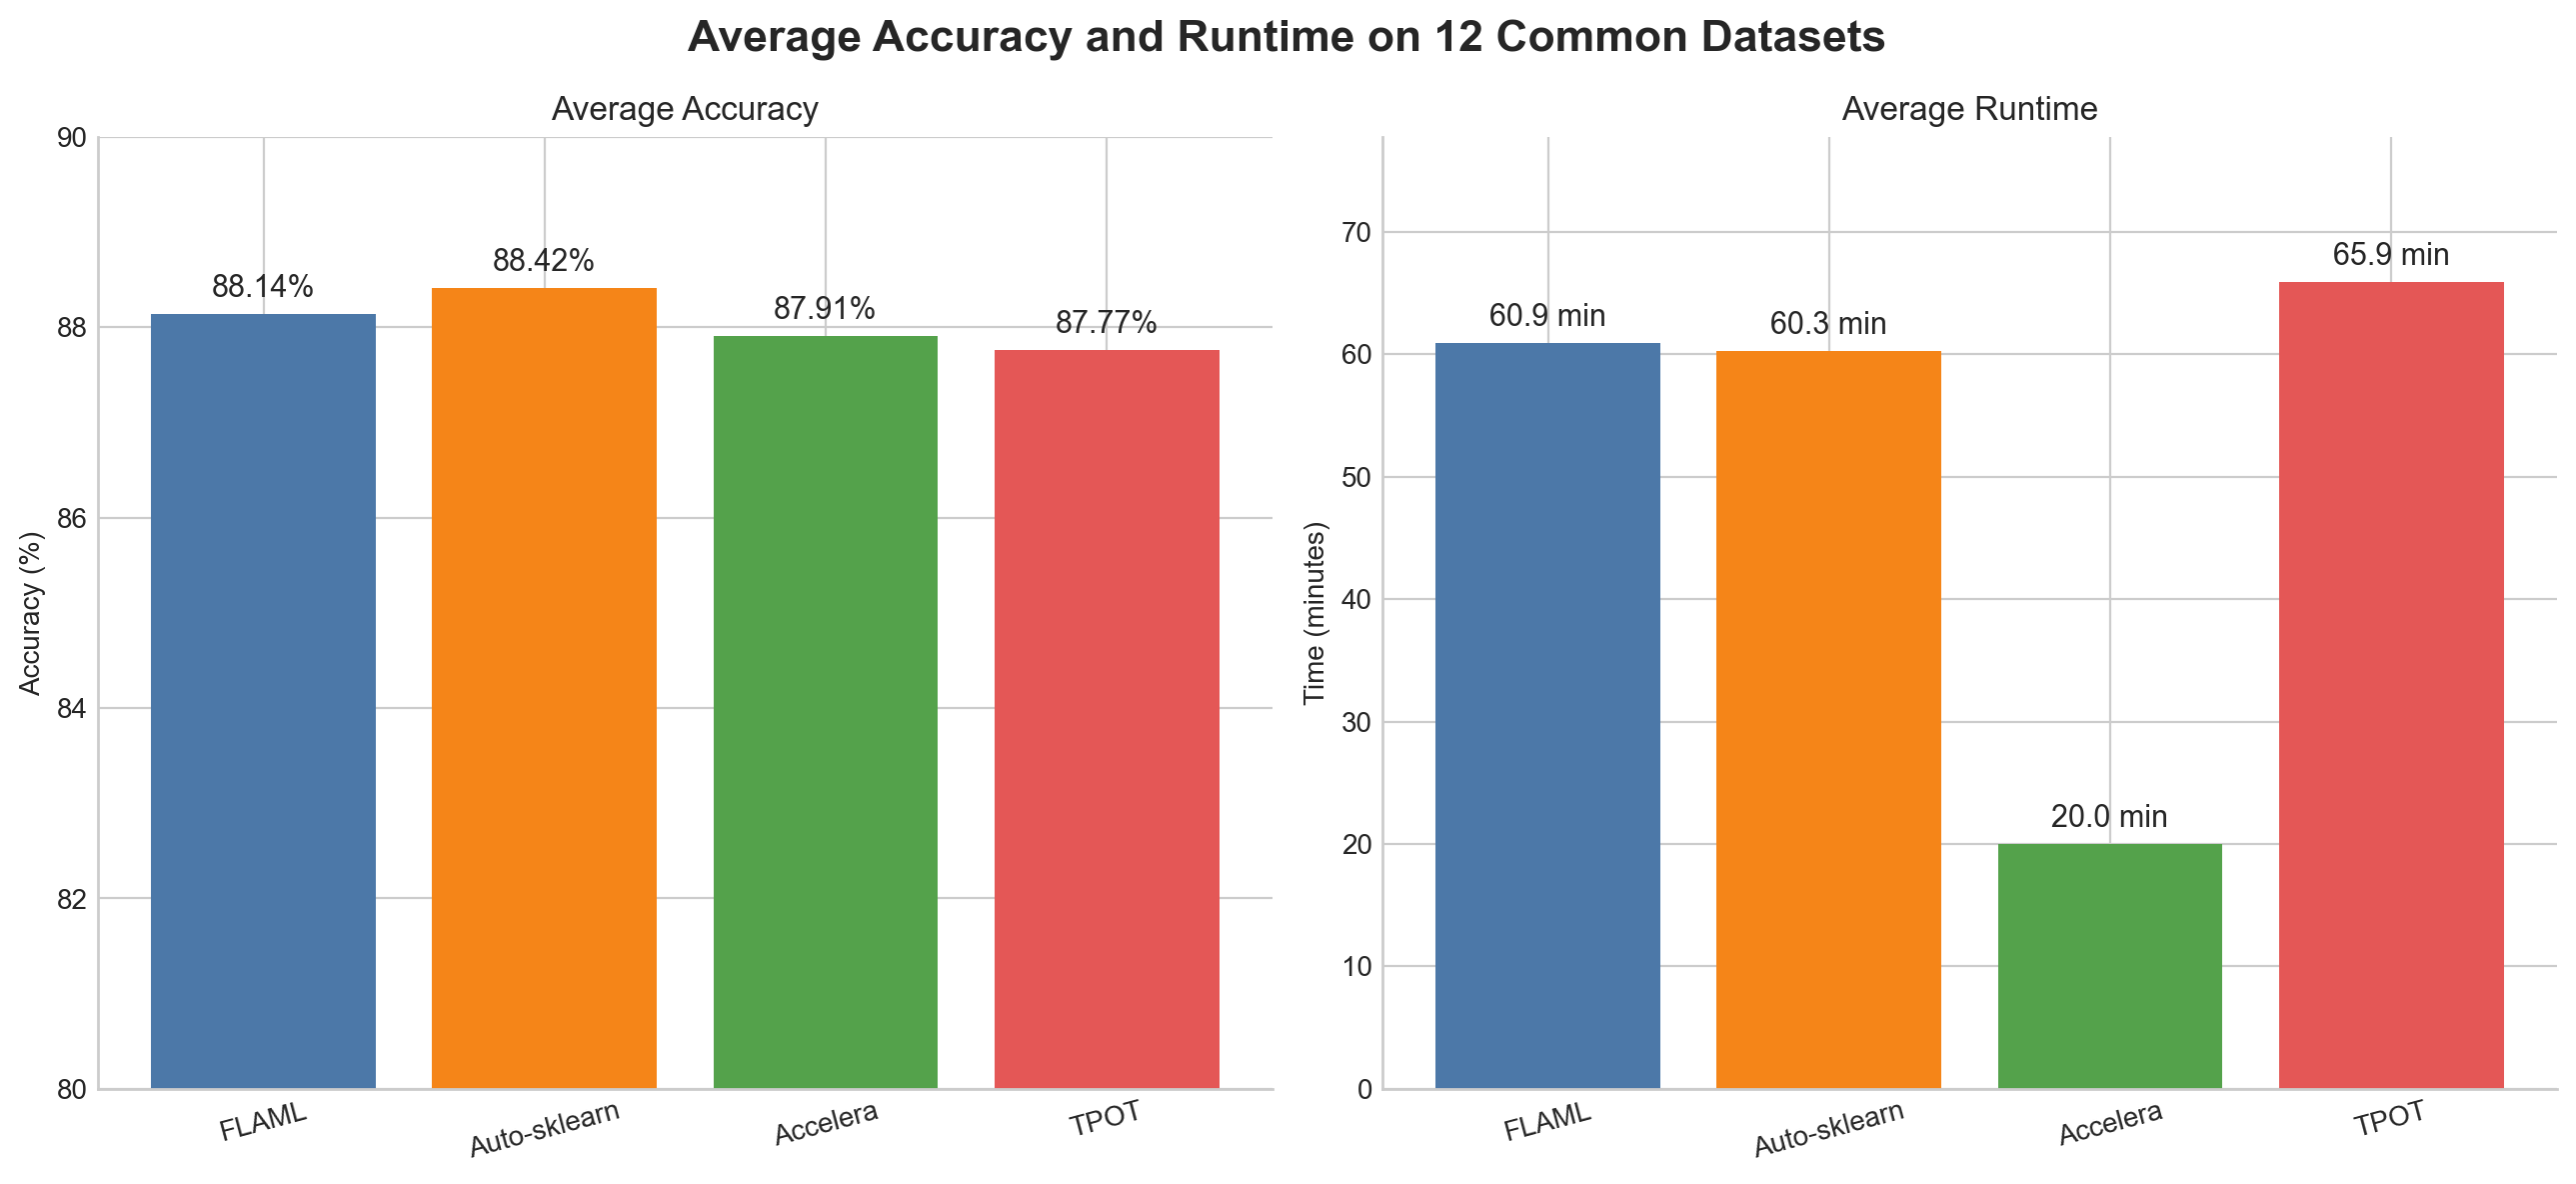
\includegraphics[width=0.78\textwidth]{../../../accelera/src/accelera_automl/benchmark_results/figures/classification/average_accuracy_time.png}
\caption{Mean classification accuracy and runtime for the evaluated systems.}
\label{fig:classification-average}
\end{figure}

\begin{figure}[H]
\centering
\begin{minipage}{0.49\textwidth}
  \centering
  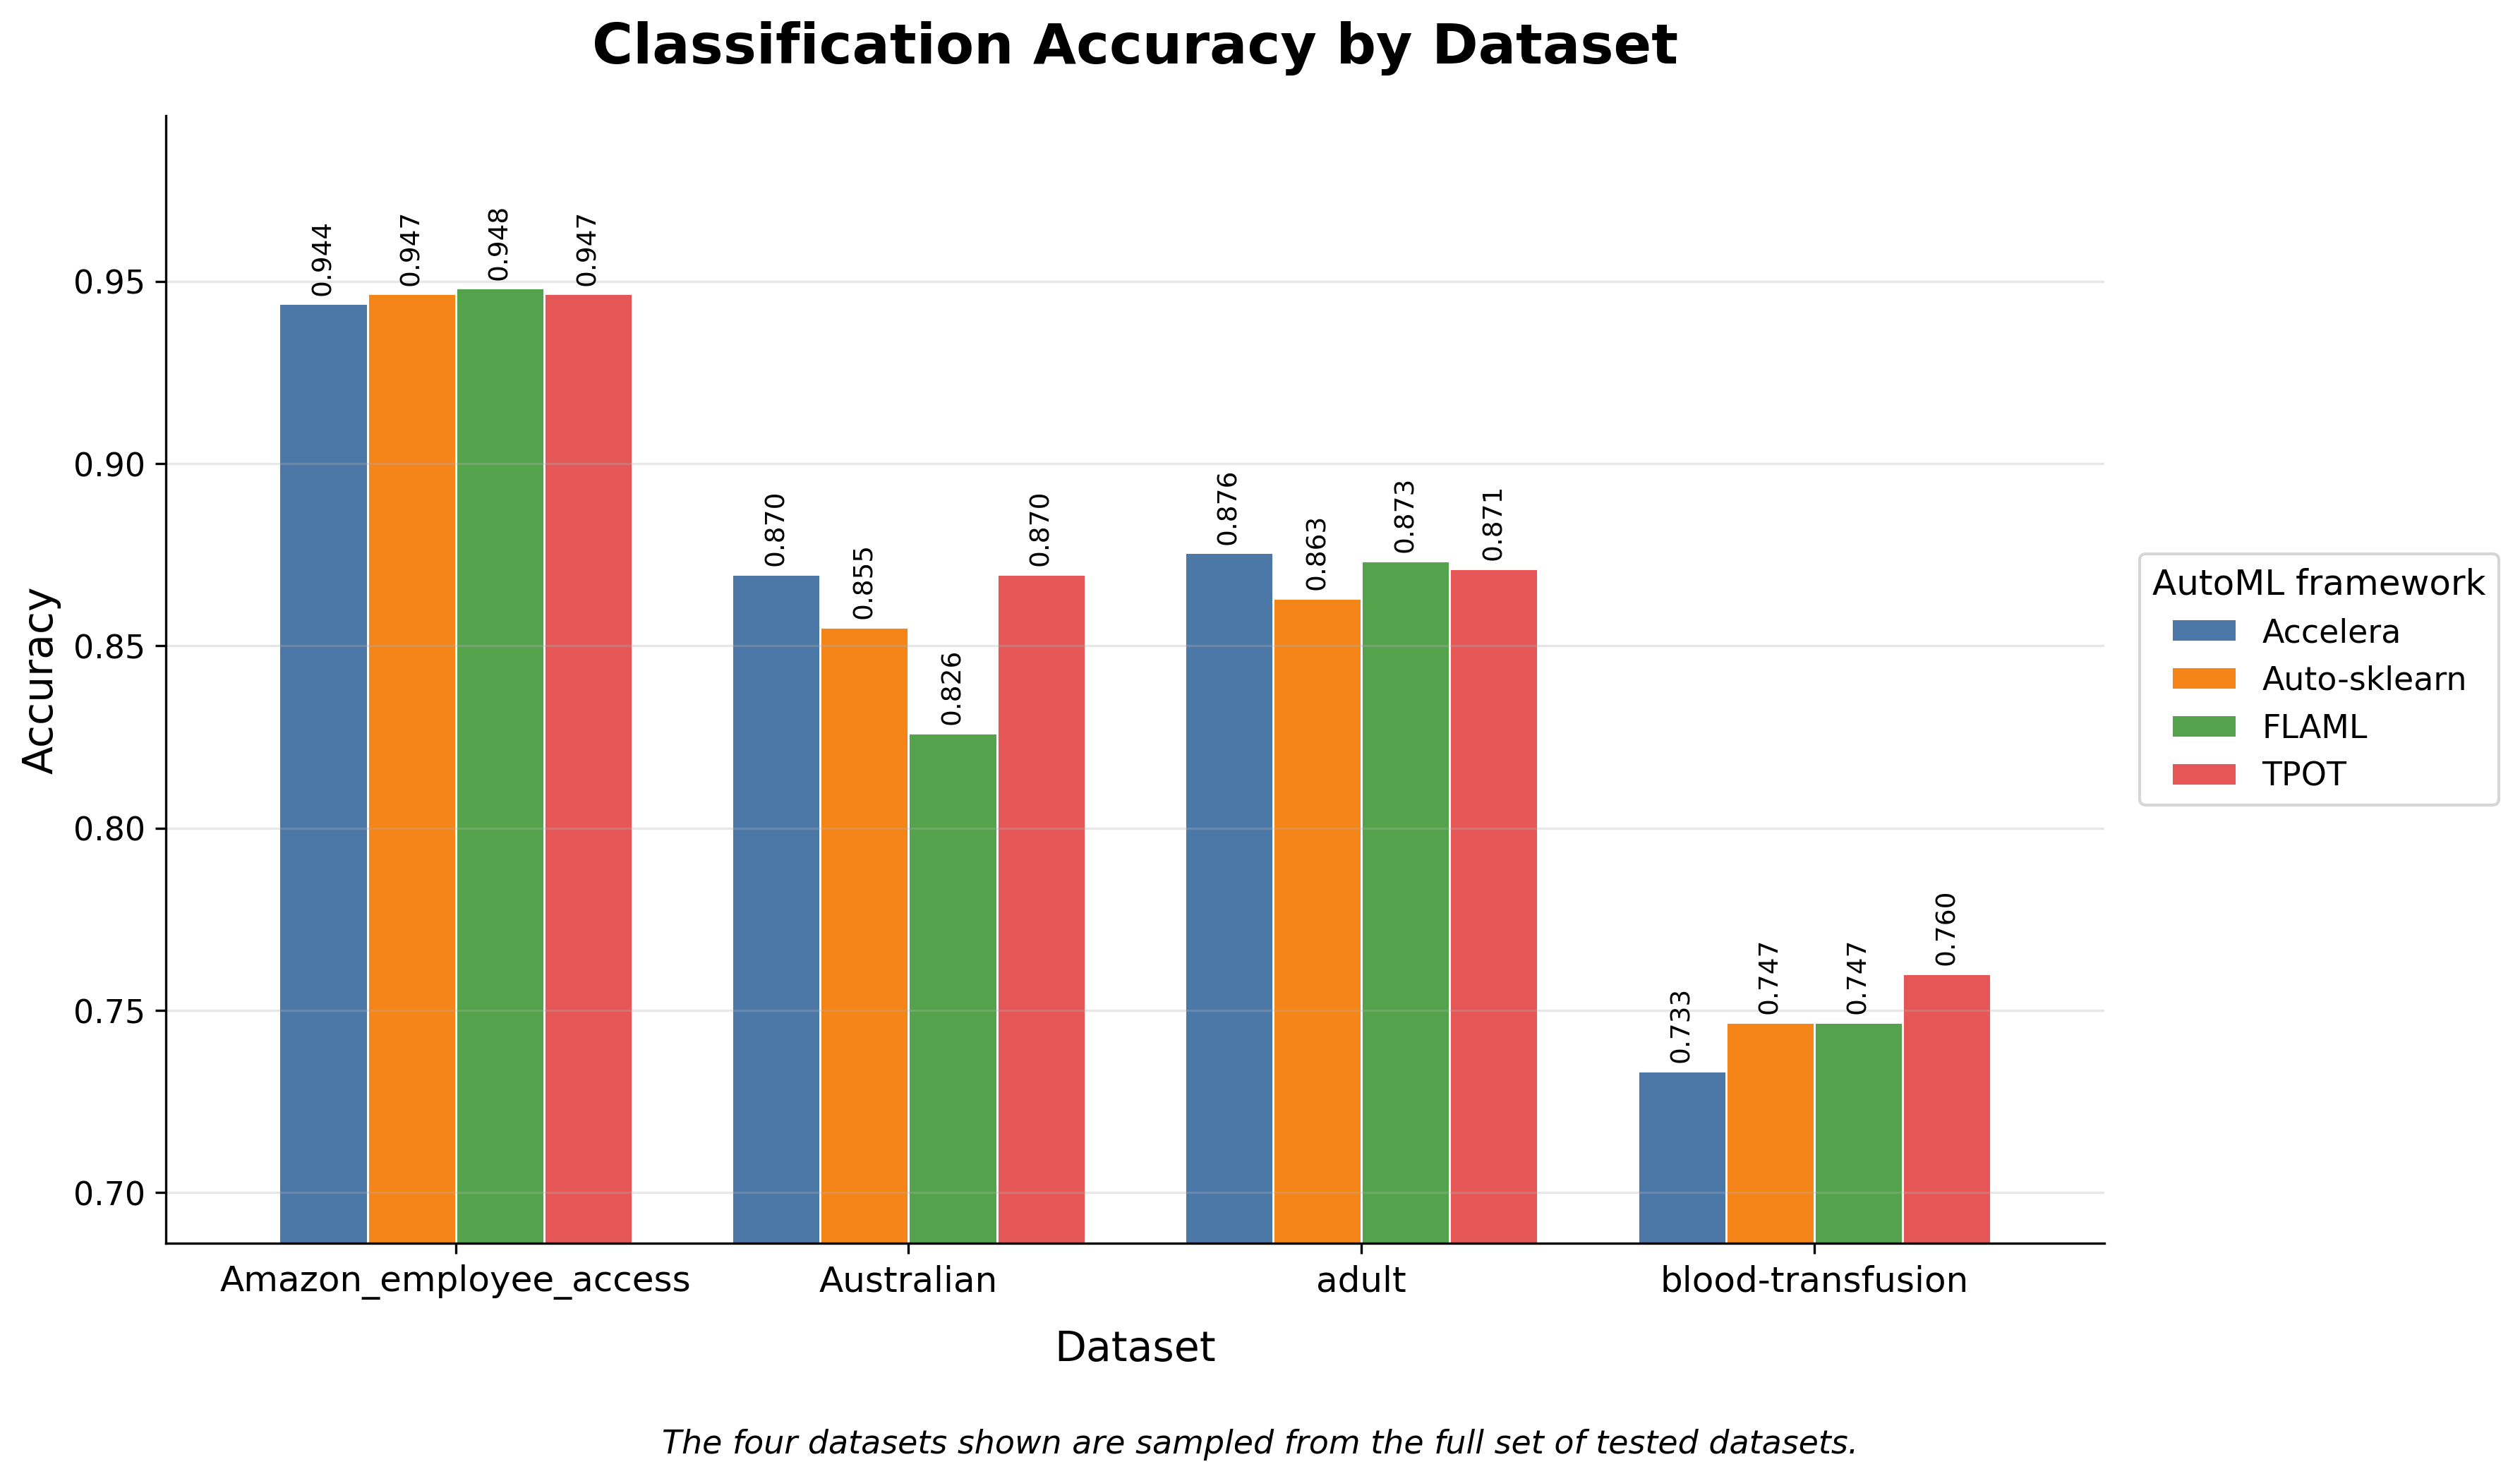
\includegraphics[width=\linewidth]{../../../accelera/src/accelera_automl/benchmark_results/figures/classification/thesis_4_datasets_accuracy_bar.png}
  \textbf{(a)} Accuracy
\end{minipage}
\begin{minipage}{0.49\textwidth}
  \centering
  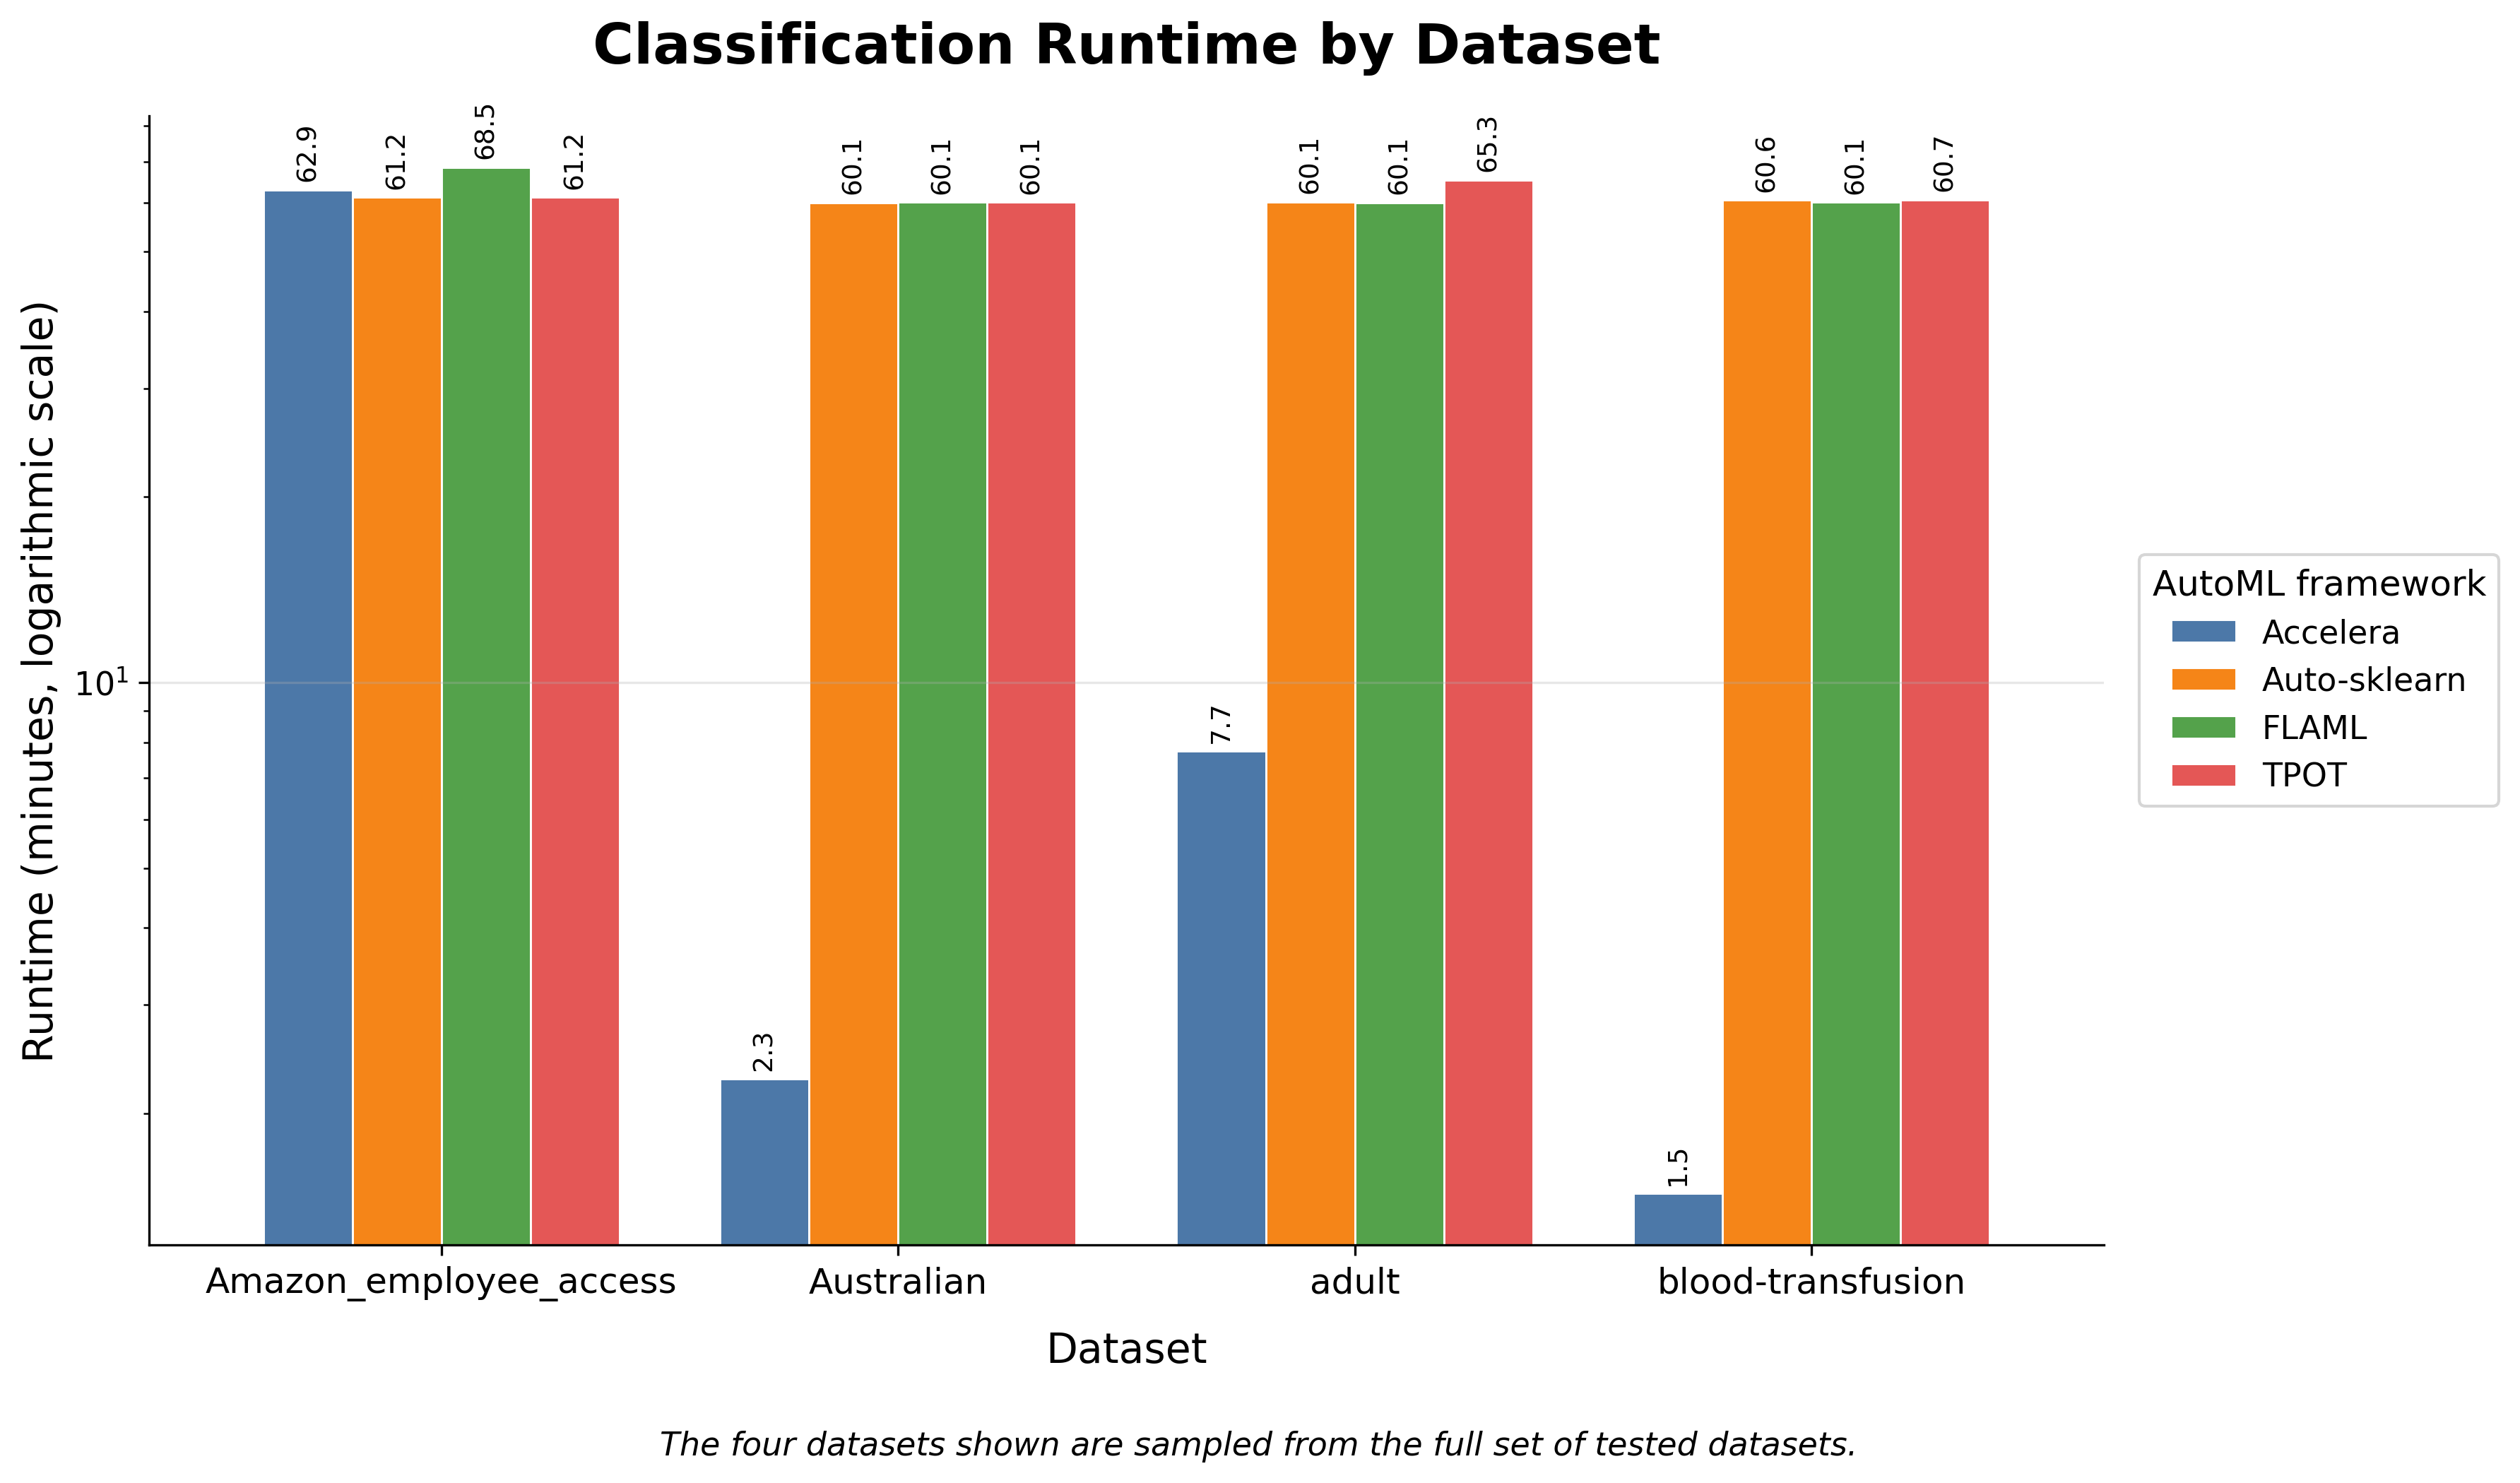
\includegraphics[width=\linewidth]{../../../accelera/src/accelera_automl/benchmark_results/figures/classification/thesis_4_datasets_duration_bar.png}
  \textbf{(b)} Duration
\end{minipage}
\caption{Per-dataset classification accuracy and duration on common datasets.}
\label{fig:classification-common}
\end{figure}

\section{Regression Results}

Table~\ref{tab:regression-results} reports the updated regression summary over
ten datasets. Auto-sklearn obtained the highest mean $R^2$ at 0.5609, followed
closely by TPOT at 0.5592. Accelera reached 0.5294 and recorded the lowest mean
runtime at 892.64 seconds, compared with 1,820--1,864 seconds for the competing
systems. Accelera also achieved six speed wins, the most of any evaluated
system.

\begin{table}[H]
\centering
\caption{Updated regression benchmark summary over ten datasets.}
\label{tab:regression-results}
\small
\resizebox{\textwidth}{!}{%
\begin{tabular}{lrrrrrrrr}
\toprule
System & Mean $R^2$ & Median $R^2$ & Mean time (s) & $R^2$ wins & RMSE wins & MAE wins & Speed wins \\
\midrule
Auto-sklearn & 0.560947 & 0.494362 & 1820.18 & 2 & 2 & 2 & 2 \\
TPOT         & 0.559238 & 0.493144 & 1849.70 & 2 & 2 & 2 & 0 \\
Accelera     & 0.529389 & 0.432577 &  892.64 & 2 & 2 & 2 & 6 \\
FLAML        & 0.522743 & 0.497530 & 1863.85 & 4 & 4 & 4 & 2 \\
\bottomrule
\end{tabular}
}
\end{table}

\begin{figure}[H]
\centering
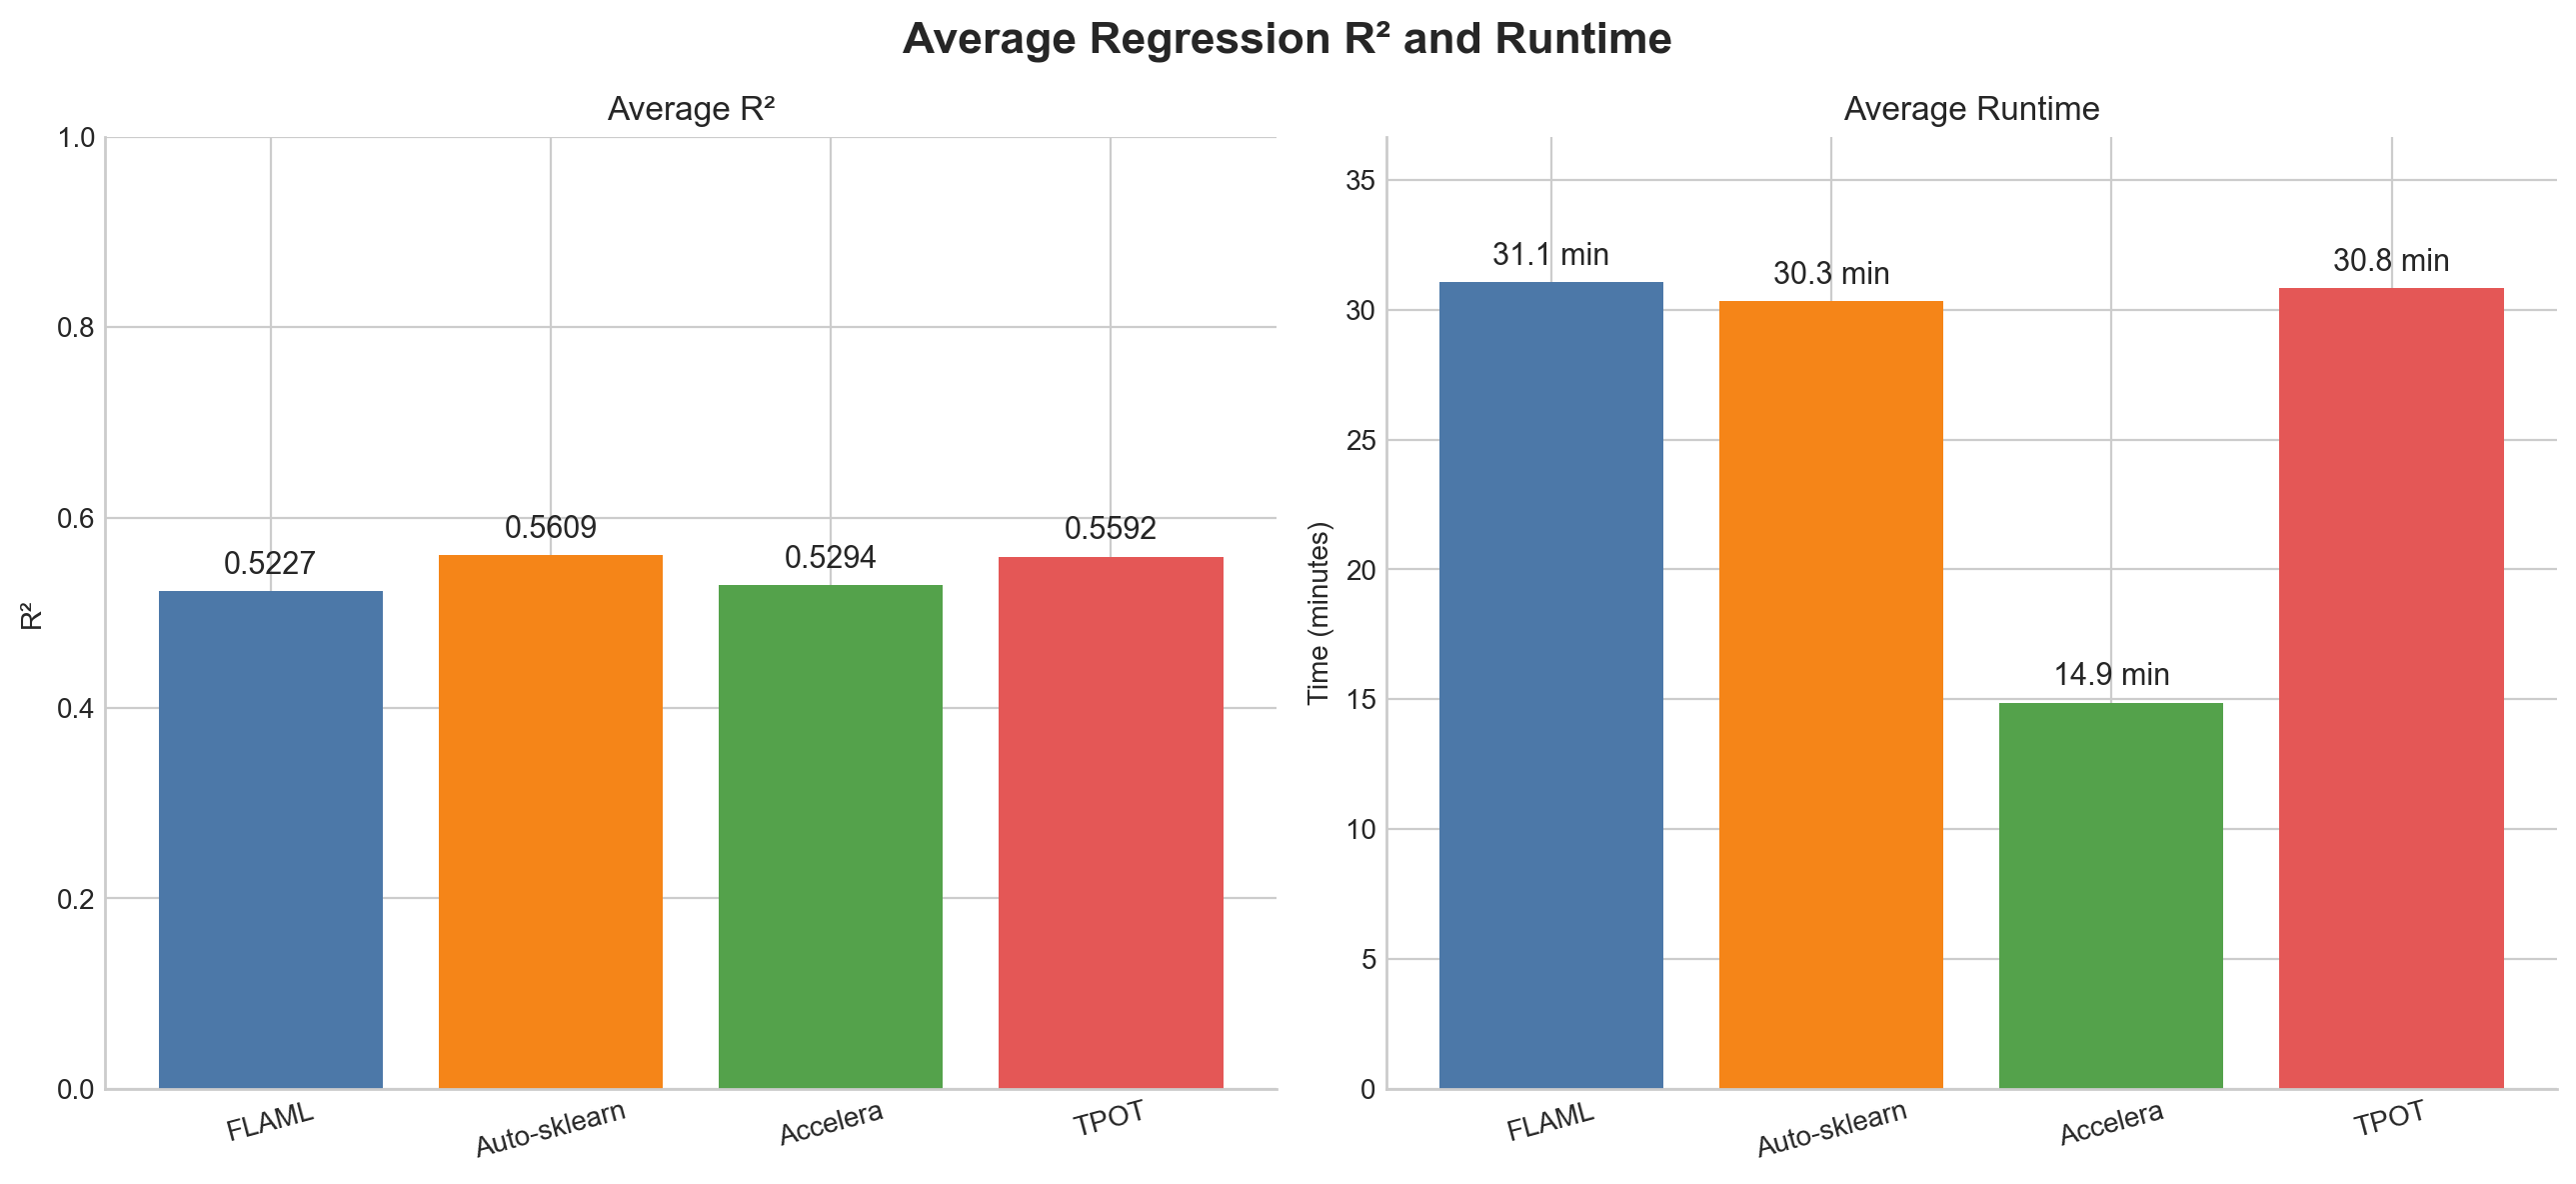
\includegraphics[width=0.78\textwidth]{../../../accelera/src/accelera_automl/benchmark_results/figures/regression/reg_average_r2_time.png}
\caption{Mean regression $R^2$ and runtime for the evaluated systems.}
\label{fig:regression-average}
\end{figure}

\begin{figure}[H]
\centering
\begin{minipage}{0.49\textwidth}
  \centering
  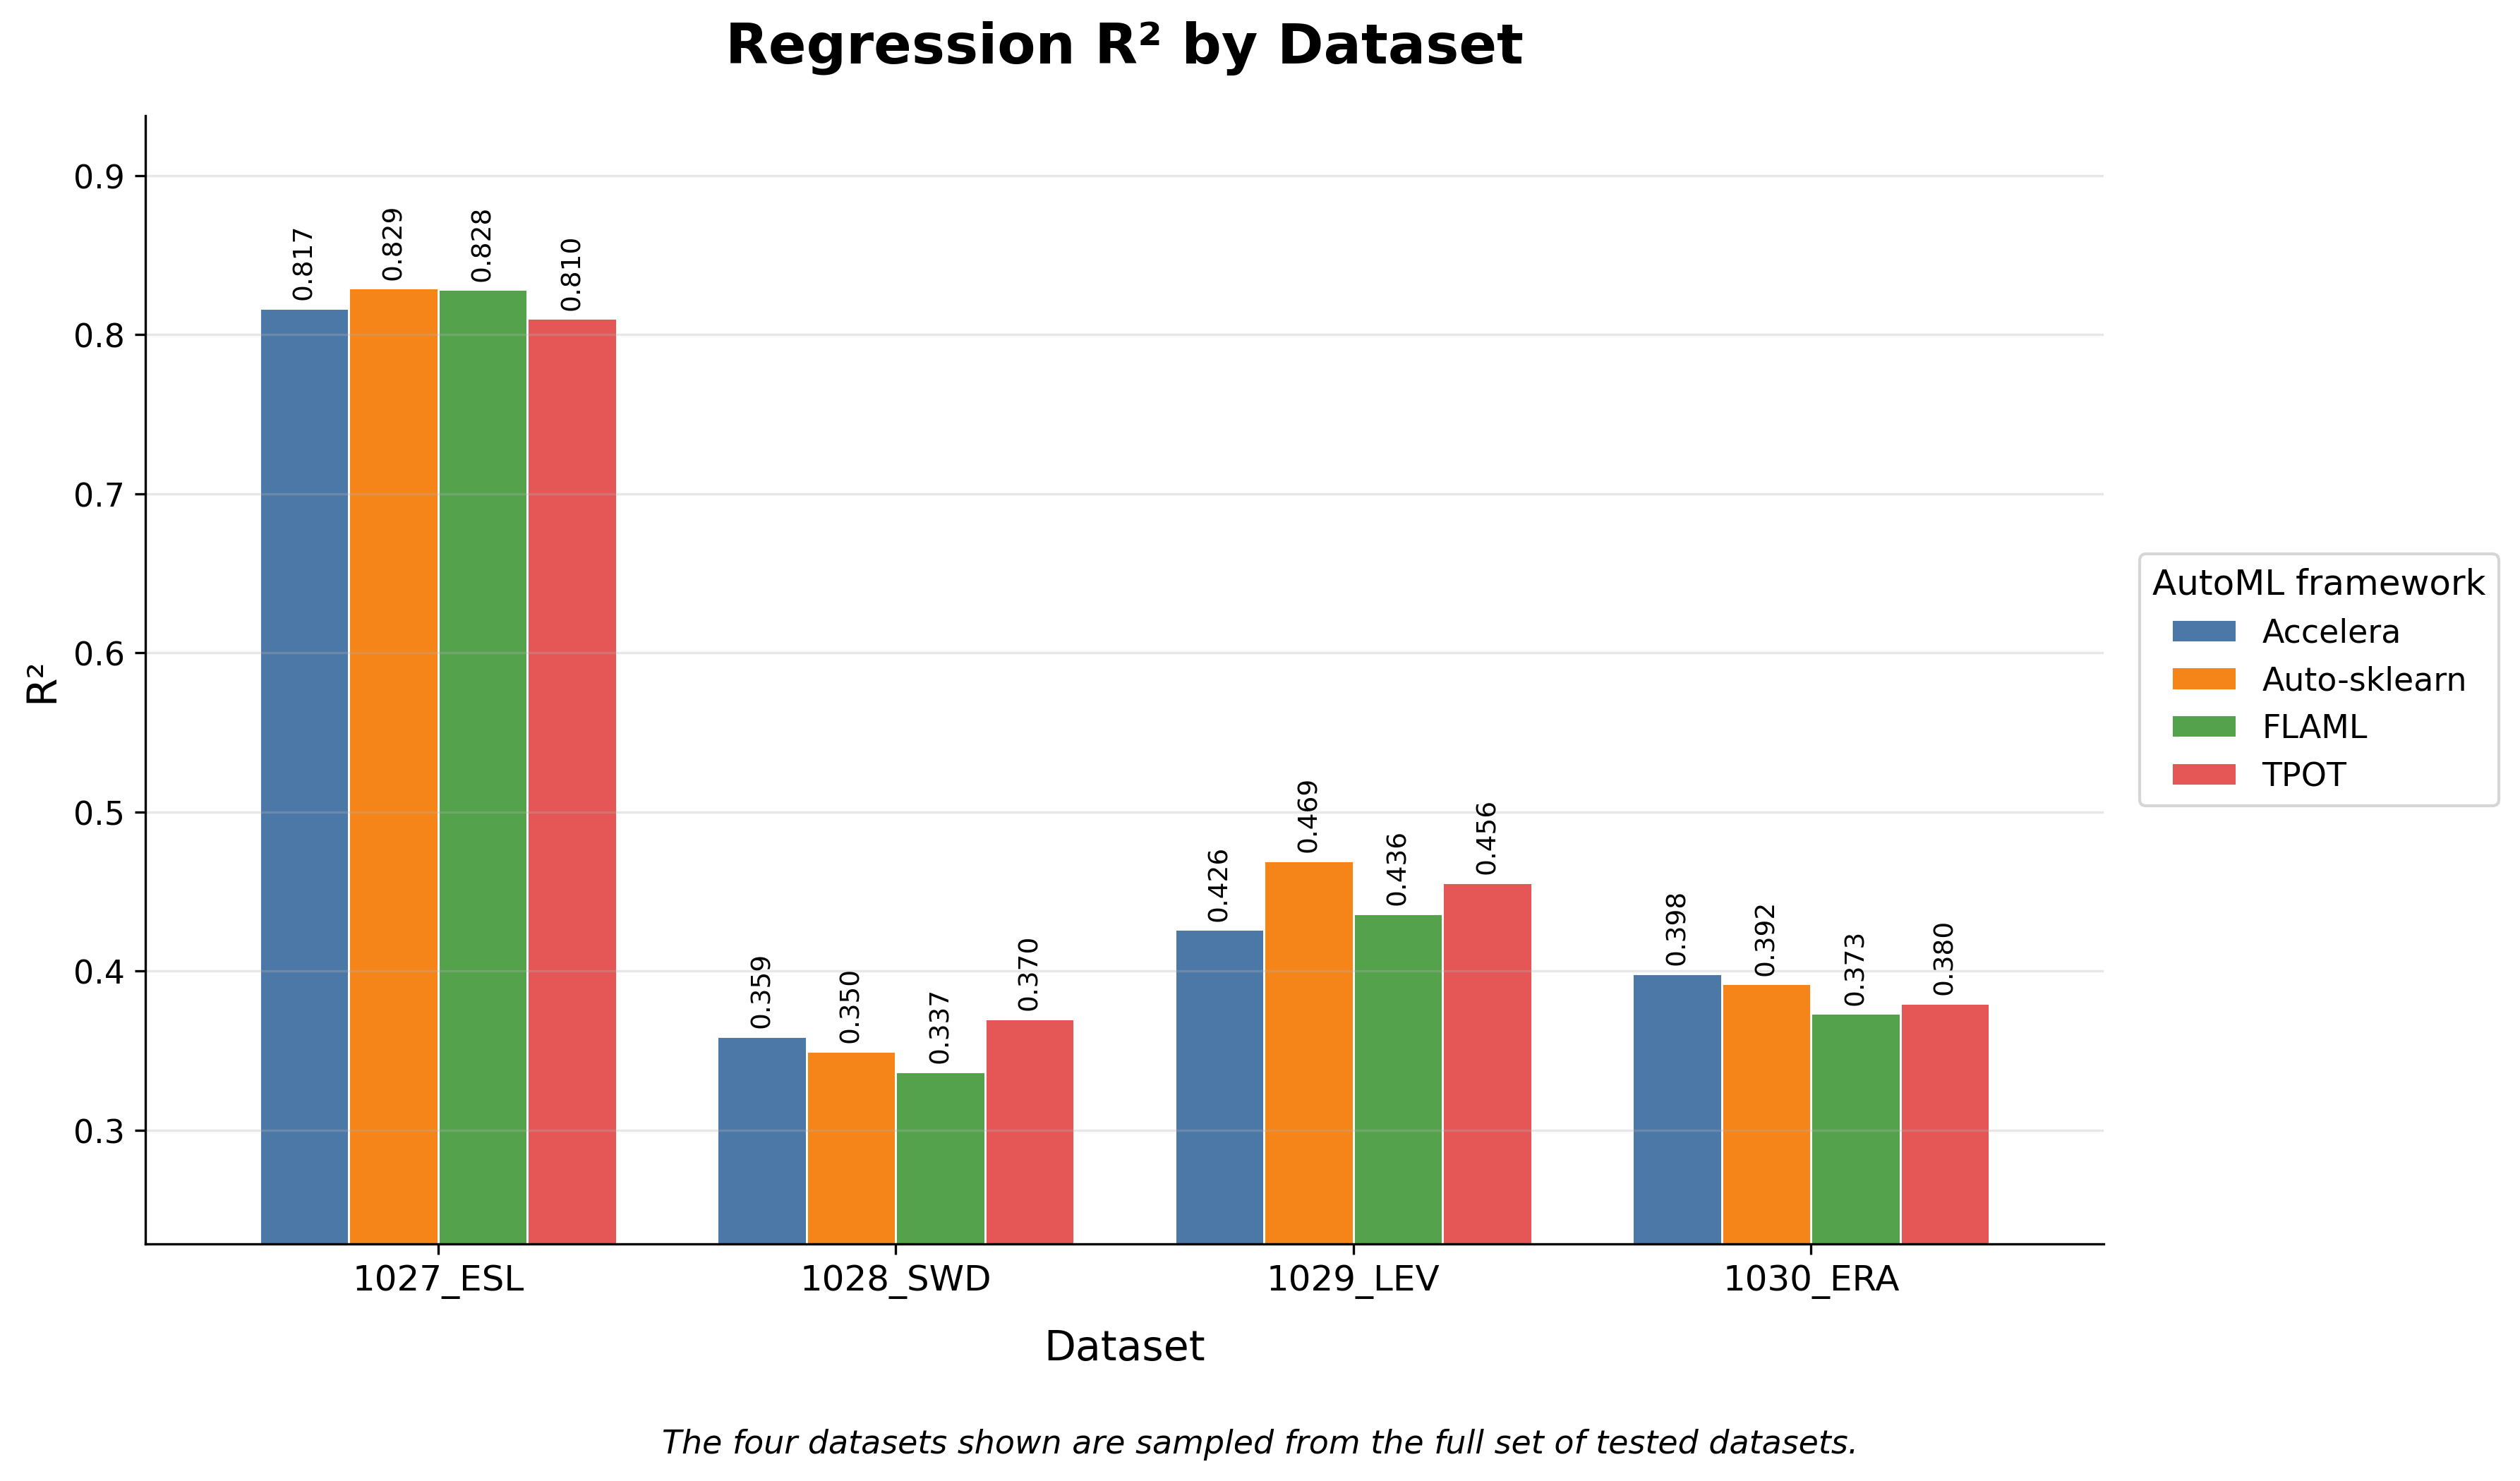
\includegraphics[width=\linewidth]{../../../accelera/src/accelera_automl/benchmark_results/figures/regression/reg_thesis_4_datasets_r2_bar.png}
  \textbf{(a)} $R^2$
\end{minipage}
\begin{minipage}{0.49\textwidth}
  \centering
  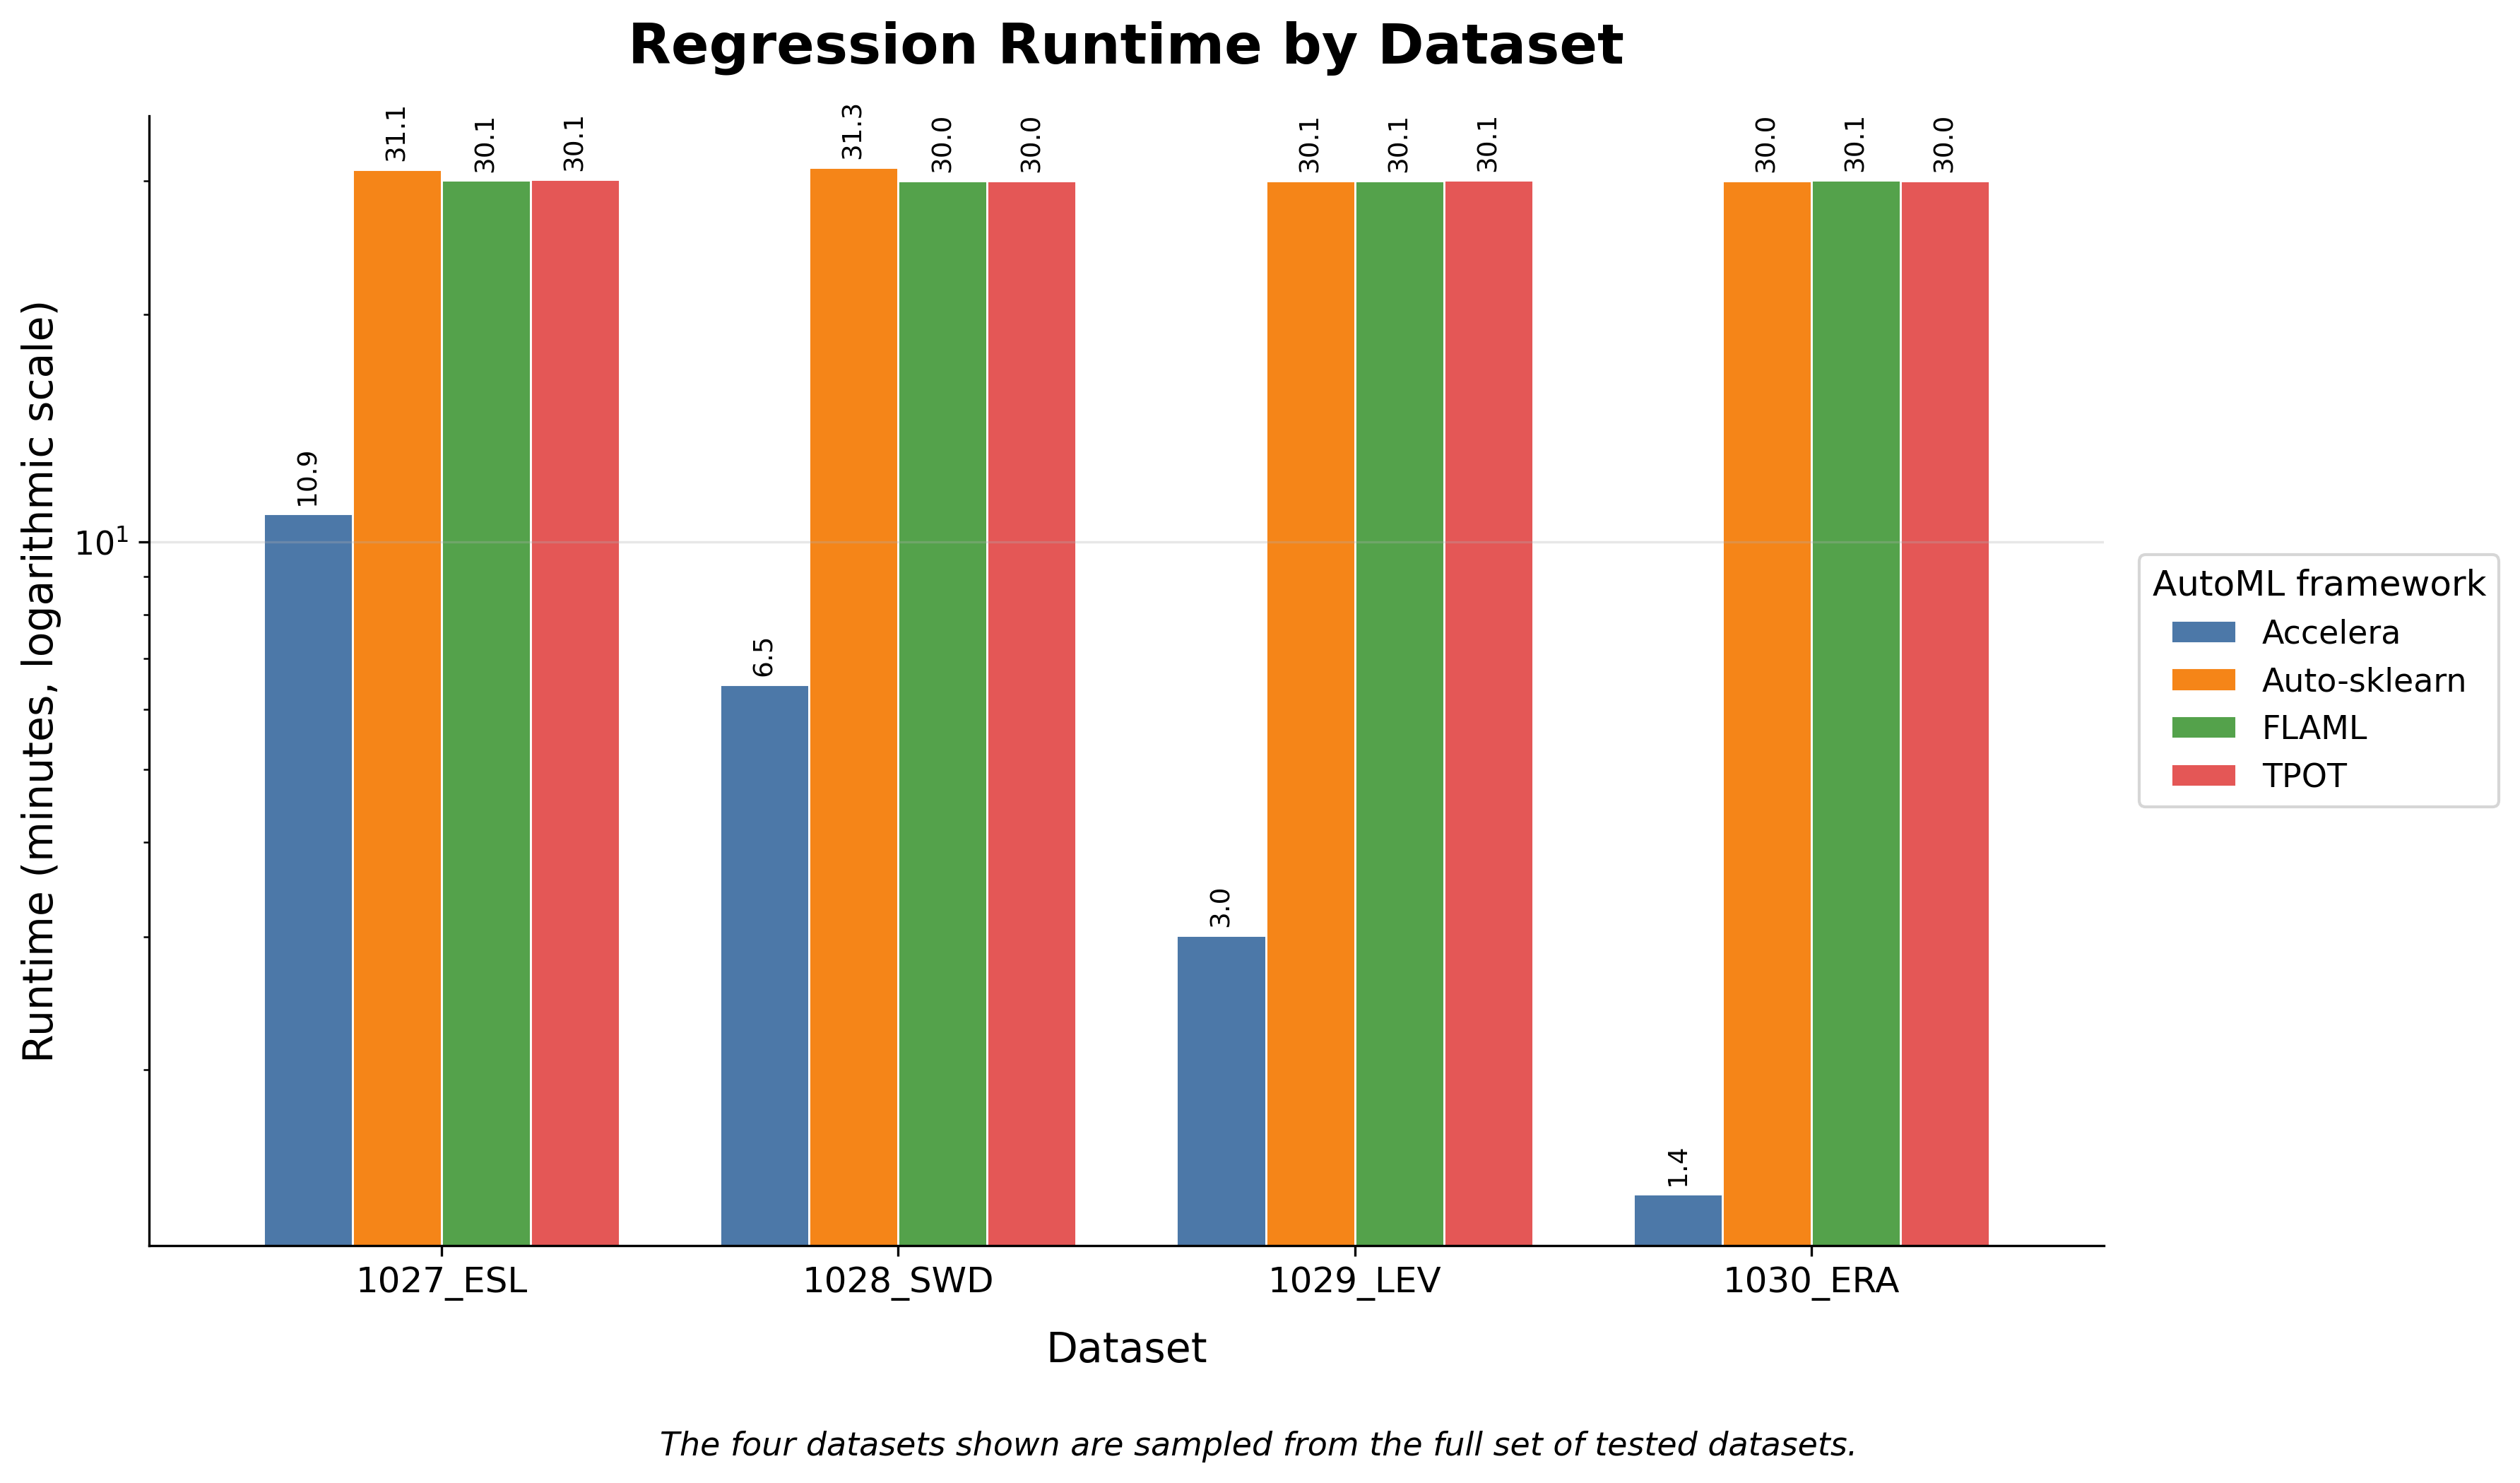
\includegraphics[width=\linewidth]{../../../accelera/src/accelera_automl/benchmark_results/figures/regression/reg_thesis_4_datasets_duration_bar.png}
  \textbf{(b)} Duration
\end{minipage}
\caption{Per-dataset regression $R^2$ and duration on common datasets.}
\label{fig:regression-common}
\end{figure}

\section{Result Reproduction}

The figures, aggregate CSV summaries, and available raw outputs are stored
under \modulepath{accelera/src/accelera\_automl/benchmark\_results}. Detailed
environment preparation and benchmark commands are documented in the
\modulepath{setup/reproduce\_results.md} file in that directory. A public
reproduction repository will be provided at
\url{https://github.com/EDIT-ME/accelera-benchmark-reproduction}; this
placeholder URL should be replaced with the final repository link before
publication.

\section{Threats to Validity}

The current results use a single benchmark fold, so they do not quantify
variation across repeated train/test splits or random seeds. Runtime is also
sensitive to hardware, operating-system load, framework startup overhead, and
timeout handling. Finally, aggregate means can conceal dataset-level failures
or missing measurements. Consequently, the tables support a comparison of the
recorded runs but should not be interpreted as a universal ranking of AutoML
systems. Repeated runs on controlled hardware and explicit reporting of failed
tasks would strengthen the evaluation.

\section{Chapter Summary}

Across the stored experiments, Accelera achieved predictive results close to
the strongest competing framework while requiring markedly less mean runtime.
The classification results show a small accuracy difference relative to
Auto-sklearn, and the regression results show a modest $R^2$ difference
relative to Auto-sklearn, accompanied in both cases by substantial runtime
reductions.
The complete stored artifacts and reproduction instructions are retained with
the implementation so that the reported measurements can be inspected and
rerun.

% Discussion, conclusion, and future-work chapters are reserved for a later
% revision.

\begin{thebibliography}{99}

\bibitem{autoweka}
Chris Thornton, Frank Hutter, Holger H. Hoos, and Kevin Leyton-Brown.
\newblock Auto-WEKA: Combined selection and hyperparameter optimization of
classification algorithms.
\newblock In \emph{Proceedings of the 19th ACM SIGKDD International Conference
on Knowledge Discovery and Data Mining}, 2013.

\bibitem{autosklearn}
Matthias Feurer, Aaron Klein, Katharina Eggensperger, Jost Springenberg,
Manuel Blum, and Frank Hutter.
\newblock Efficient and robust automated machine learning.
\newblock In \emph{Advances in Neural Information Processing Systems}, 2015.

\bibitem{tpot}
Randal S. Olson, Nathan Bartley, Ryan J. Urbanowicz, and Jason H. Moore.
\newblock Evaluation of a tree-based pipeline optimization tool for automating
data science.
\newblock In \emph{Applications of Evolutionary Computation}, 2016.

\bibitem{flaml}
Chi Wang, Qingyun Wu, Markus Weimer, and Erkang Zhu.
\newblock FLAML: A fast and lightweight AutoML library.
\newblock In \emph{Proceedings of Machine Learning and Systems}, 2021.

\bibitem{autogluon}
Nick Erickson et al.
\newblock AutoGluon-Tabular: Robust and accurate AutoML for structured data.
\newblock \emph{arXiv preprint arXiv:2003.06505}, 2020.

\bibitem{smac}
Frank Hutter, Holger H. Hoos, and Kevin Leyton-Brown.
\newblock Sequential model-based optimization for general algorithm
configuration.
\newblock In \emph{Learning and Intelligent Optimization}, 2011.

\bibitem{randomsearch}
James Bergstra and Yoshua Bengio.
\newblock Random search for hyper-parameter optimization.
\newblock \emph{Journal of Machine Learning Research}, 13:281--305, 2012.

\bibitem{stacking}
David H. Wolpert.
\newblock Stacked generalization.
\newblock \emph{Neural Networks}, 5(2):241--259, 1992.

\end{thebibliography}

\end{document}
